% This is LLNCS.DEM the demonstration file of
% the LaTeX macro package from Springer-Verlag
% for Lecture Notes in Computer Science,
% version 2.4 for LaTeX2e as of 16. April 2010
%
\documentclass{llncs}
%
\usepackage{makeidx}  % allows for indexgeneration
\usepackage{amssymb}
\usepackage{amsmath}
\usepackage{algorithmic,eqparbox,array}
\usepackage{algorithm}
\usepackage{graphicx}
\usepackage{listings}
\usepackage{color}
\usepackage{multirow,booktabs,ctable,array}


    \definecolor{listcomment}{rgb}{0.0,0.5,0.0}
    \definecolor{listkeyword}{rgb}{0.0,0.0,0.5}
    \definecolor{listnumbers}{gray}{0.65}
    \definecolor{listlightgray}{gray}{0.955}
    \definecolor{listwhite}{gray}{1.0}


%\floatname{algorithm}{Procedure}
\renewcommand{\algorithmicrequire}{\textbf{Input:}}
\renewcommand{\algorithmicensure}{\textbf{Output:}}
\renewcommand{\algorithmiccomment}[1]{\hfill\eqparbox{COMMENT}{// #1}}
%
\begin{document}
%
\frontmatter          % for the preliminaries
%

\mainmatter              % start of the contributions
%
\title{Advanced Normalization Tools for Cardiac Motion Correction}
%
\titlerunning{}  % abbreviated title (for running head)
%                                     also used for the TOC unless
%                                     \toctitle is used
%
\author{Nicholas J. Tustison \and Yang Yang \and Michael Salerno}

\authorrunning{N. J. Tustison, Y. Yang, M. Salerno} % abbreviated author list (for running head)
\institute{University of Virginia, Charlottesville VA 22903, USA
}

\maketitle              % typeset the title of the contribution

\begin{abstract}
We present our submission to the STACOM 2014 MoCo challenge for 
motion correction of dynamic contrast myocardial perfusion
MRI.  Our submission is based on the publicly available Advanced
Normalization Tools (ANTs) specifically tailored for this problem
domain.  We provide a brief description with actual code calls
to facilitate reproducibility.  Time plots based on the
validation methodology of \cite{pack2010} are also illustrated
to determine clinically relevant performance levels.
\keywords{ANTs, image registration, motion estimation, myocardial perfusion}
\end{abstract}

\section{Introduction}

Motion correction for dynamic contrast MR myocardial perfusion is of significant
research interest and has resulted in several techniques generally characterized as
rigid or non-rigid image registration-based.  To bring together interested 
researchers for discussion and comparison of methods for correction of motion
artefacts and the development of performance benchmarks of such techniques, 
the STACOM 2014 workshop committee organized a motion correction challenge 
to be held in conjunction with MICCAI 2014.

We describe the submission of our non-rigid motion correction approach
below which is both publicly available and open source.  This facilitates 
reproducibility for other researchers who wish to investigate the methods
proposed and perhaps formulate configurations which improve existing
performance levels.
\section{Methods}

We used the Advanced Normalization Tools (ANTs)
package as the basis of our motion correction estimation framework as it provides 
a suite of utilities for image preprocessing and registration which have exhibited 
excellent performance in a variety of applications and challenges.  For example, 
the popular Symmetric Normalization (SyN) algorithm \cite{avants2008,avants2011}
performed well in a recent evaluation of popular deformable registration 
algorithms on human brain images \cite{klein2009}.  Similarly, ANTs image registration and other 
capabilities were instrumental in recent MICCAI challenge performances including 
the lung-based EMPIRE10 (pulmonary CT) \cite{murphy2011} and BRATS2013 
(multimodal MRI, brain tumor) \cite{menze2014}.

Normalization to the reference frame employs a pairwise registration strategy
whereby each image is registered to its successive temporal neighbor using 
a recently developed SyN variation where the smoothing kernel is based on 
B-splines \cite{tustison2013}.  One of the benefits of SyN is that it yields both 
the forward and inverse transforms between images $I$ and $J$, which we denote
as $I \underset{b}{\leftrightsquigarrow} J$ (where `$b$' denotes ``B-spline SyN'').
Note that the image of the last time frame is registered to the image at the 
first time frame.  Thus, to transform any image, $I_t$, at time point, $t$, to the 
reference image, $I_R$, temporally located at time, $t=r$, we simply concatenate 
the transforms either forwards
\begin{align}
I_R  \underset{b_r}{\leftrightsquigarrow} \underset{b_{r+1}}{\leftrightsquigarrow} \cdots
      \underset{b_{t-2}}{\leftrightsquigarrow}\underset{b_{t-1}}{\leftrightsquigarrow} I_t
\end{align}
or backwards
\begin{align}
I_R  \underset{b_{r-1}}{\leftrightsquigarrow} \underset{b_{r-2}}{\leftrightsquigarrow} \cdots
      \underset{b_{t+1}}{\leftrightsquigarrow}\underset{b_t}{\leftrightsquigarrow} I_t.
\end{align}
By concatenating transforms, only a single
interpolation is performed for each normalization to the reference frame.  
%This flexibility 
%permits a brute-force search strategy for the optimal ``split time index'' which we discuss
%later.  

Given the temporal image variability and other confounds (e.g., noise), 
a multivariate image registration strategy was employed.  Conventional
image registration approaches are often limited to a single metric choice
with a single ``fixed'' and ``moving'' image pair.  In contrast, we 
use multiple image
pairs and corresponding metrics which is made possible by recent 
developmental work to the Insight Toolkit \cite{avants2014}.  
These additional image pairs were created using several processing steps.
Preprocessing for each image included N4 bias correction to minimize low frequency
intensity variation artifacts commonly associated with MRI \cite{tustison2010}.  From each
bias corrected image we created the following two images:  (1) an image derived
from a noise reduction filtering procedure meant to preserve structure 
\cite{smith1997} known as ``SUSAN'' from the FMRIB Software Library (FSL)%
\footnote{
http://fsl.fmrib.ox.ac.uk/fsl/fslwiki/
}
and (2) a Laplacian-based edge-detection image
derived from the SUSAN image.  A sample set of these images for one of the MoCo
data is found in Figure \ref{fig:subject9}.

\begin{figure}
\centering
  \begin{tabular}{cccc}
    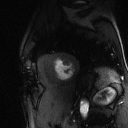
\includegraphics[width=29.5mm]{Figures/MoCo_09_Rest_23_Original.png} &
    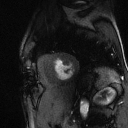
\includegraphics[width=29.5mm]{Figures/MoCo_09_Rest_23_N4.png} &
    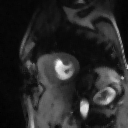
\includegraphics[width=29.5mm]{Figures/MoCo_09_Rest_23_SUSAN.png} &
    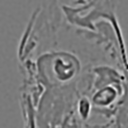
\includegraphics[width=29.5mm]{Figures/MoCo_09_Rest_23_Laplacian.png} \\
    (a) & (b) &
    (c) & (d) \\
  \end{tabular}
  \caption{Sample auxiliary images from the MoCo data set (Subject 9 (Rest): Frame 23).
           Shown are the (a) original, (b) N4 bias corrected, (c) SUSAN, and (d) Laplacian
           images.}
  \label{fig:subject9}         
\end{figure}


Each of these three sets of derived images are used to drive a deformable B-spline SyN
pairwise registration for each temporal neighboring image pair.
This process is most clearly described by the {\tt antsRegistration} program call given in Listing 
\ref{listing:antsRegistration}.%
\footnote{
In many situations, the deformable registration portion of the total alignment strategy
is preceded by one or more linear registrations (e.g., center of mass alignment, affine 
registration).  This is easily accommodated into the {\tt antsRegistration} command line
syntax.  However, for this specific problem domain, it was found that such pre-deformable
alignment steps were unnecessary.
}  
Each fixed and moving image pair was histogram
matched \cite{nyul2000} and intensity-truncated to remove extreme values.  The
choice of similarity metric for each image pair was motivated by the characteristics
of each individual set and the need to balance an aggressive alignment of strong image features 
while minimizing displacements caused by incorrect correspondences.  The N4 bias corrected
images were incorporated into the motion correction strategy since they were closest
to the original imaging data. Given the relative amount of noise, we used a neighborhood
CC metric (window radius = 6 voxels) to help mitigate the noise issue for these data which
is the default similarity metric choice used in ANTs-based image registration \cite{avants2008}.  In
contrast, as SUSAN is meant to minimize noise corruption, we used the more aggressive
Demons metric \cite{thirion1998} for the SUSAN and Laplacian image pairs.  We used
equal weighting for each image pair/similarity metric although investigation into
relative weighting schemes might increase performance levels.  A multi-resolution approach
consisting of three levels with each successive level corresponding to double the resolution
of the previous level was used with varying isotropic smoothing used at each level.  For
specific parameter choices, we refer the reader to Listing 
\ref{listing:antsRegistration}.
%In addition, we used a masking strategy to limit
%the calculation of the image similarity metric to the region immediately surrounding
%the myocardium and including the myocardial cavity.  The mask for each temporal
%image series was automatically created by performing a binary morphological dilation
%of the myocardial mask provided by the challenge organizers.  Any holes in the resulting 
%mask were filled using a binary filling operation. 

\lstset{frame = htb,
        framerule = 0.25pt,
        float,
        fontadjust,
        backgroundcolor={\color{listlightgray}},
        basicstyle = {\ttfamily\scriptsize},
        keywordstyle = {\ttfamily\color{listkeyword}\textbf},
        identifierstyle = {\ttfamily},
        commentstyle = {\ttfamily\color{listcomment}\textit},
        stringstyle = {\ttfamily},
        showstringspaces = false,
        showtabs = false,
        numbers = none,
        numbersep = 6pt,
        numberstyle={\ttfamily\color{listnumbers}},
        tabsize = 2,
        language=c++,
        floatplacement=!h,
        caption={\small {\tt antsRegistration} call used for the pairwise registration.  
        },
        captionpos=b,
        label=listing:antsRegistration
        }
\begin{lstlisting}
// Input image pairs include:
//  * N4 bias corrected
//  * Structure-preserving noise reduction (SUSAN) of N4 images
//  * Laplacian filtering of N4 images.

antsRegistration --dimensionality 2 
                 --output ${registrationPrefix} \
                 --winsorize-image-intensities [0.01,0.99] \
                 --use-histogram-matching 1 \
                 --transform BSplineSyN[0.1,2x2,0] \
                 --metric CC[${n4Fixed},${n4Moving},1,6] \
                 --metric Demons[${susanFixed},${susanMoving},1,1] \
                 --metric Demons[${laplacianFixed},${laplacianMoving},1,1] \
                 --convergence [100x70x50,1e-8,10] \
                 --shrink-factors 4x2x1 \
                 --smoothing-sigmas 1x0.5x0vox
\end{lstlisting}

Once all the pairwise transforms are generated between each set of temporal 
neighbors, we normalize all the original images to the reference frame
by concatenating all the transforms using the program {\tt antsApplyTransforms}
which performs only a single interpolation per normalization regardless of
the number of transforms specified.

\section{Evaluation}

As described by the challenge organizers:

\begin{quote}
{\it
We will validate the motion correction algorithms based on flow indices. 
That is, the registered datasets will be processed to
\begin{itemize}
\item create time curves for each of 6 tissue regions,
\item create an arterial input function (AIF) from the automatically determined 
blood pool curves within the endocardial border,
\item subtract off the average of the initial pre-contrast frames and 
normalize by estimated coil sensitivity differences so that the time curves 
are proportional to gadolinium concentration, and
\item fit the data to a compartment model to obtain myocardial blood flow MBF in 
ml/g/min  \cite{pack2010}.
\end{itemize}
The score will be the sum of squared differences of the Myocardial Blood 
Flow (MBF) index with the registration method, compared to MBF of a 
pseudo-gold standard obtained from manually drawn contours from experienced 
analysts.}%
\footnote{
http://www.cardiacatlas.org/web/stacom2014/moco-validation
}
\end{quote}
Implementation of the validation methodology was provided by the workshop 
organizers which were applied to all motion-corrected 10 gated image sets and the 
single ungated data set.  The resulting time curves and model fits are
given in Figures \ref{fig:gated1}, \ref{fig:gated2}, and \ref{fig:ungated}.

\begin{figure}
 \makebox[\textwidth][c]{
   \begin{tabular}{ccccc}
    {} & \multicolumn{2}{c}{\bf Rest} &  \multicolumn{2}{c}{\bf Stress} \\
    \rotatebox{90}{\bf \,\,\,\,\,\,\,\,\,\,\,\,\,MoCo\_01} & 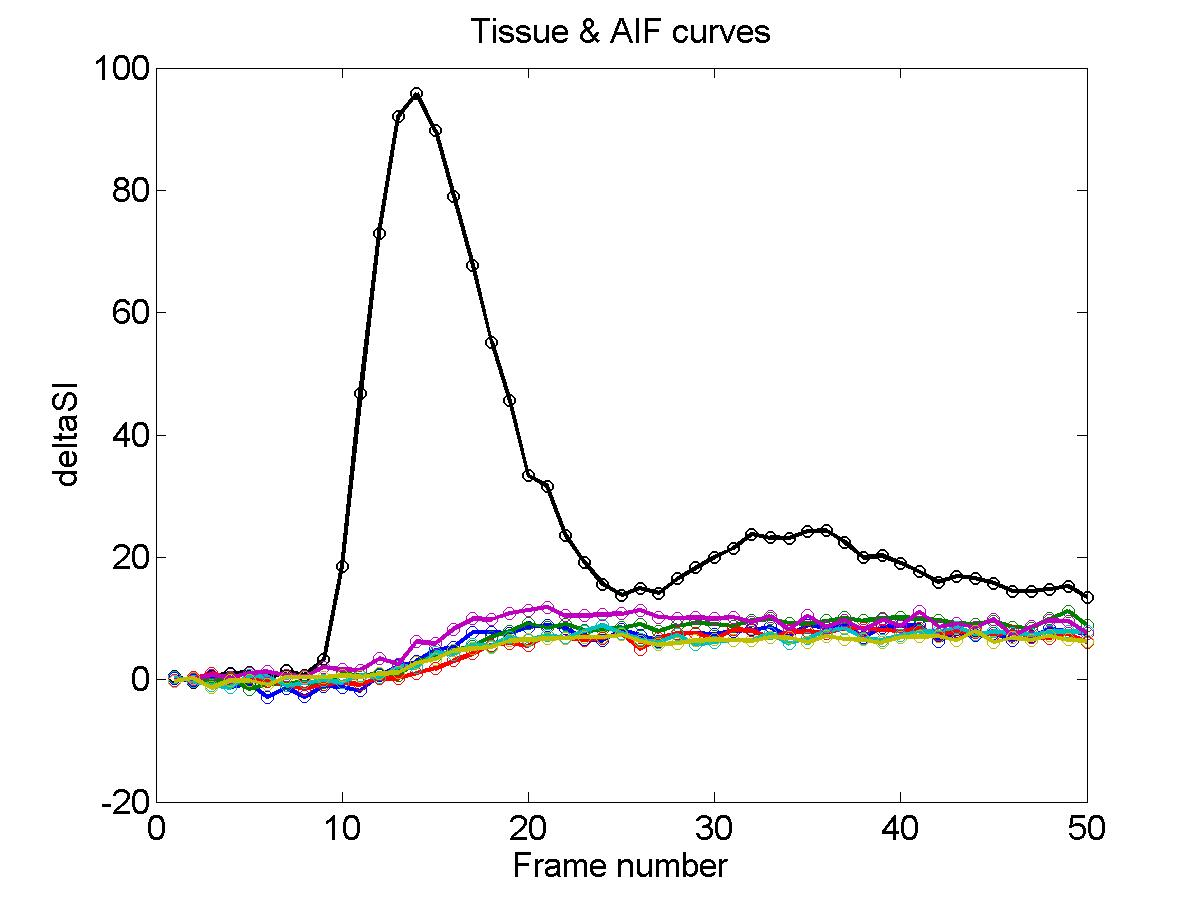
\includegraphics[width=40mm]{Figures/Results_jpg_DZnomask/MoCo_01_DZNoMask_Rest_Curve.jpg} 
    \hspace{-5mm} &
    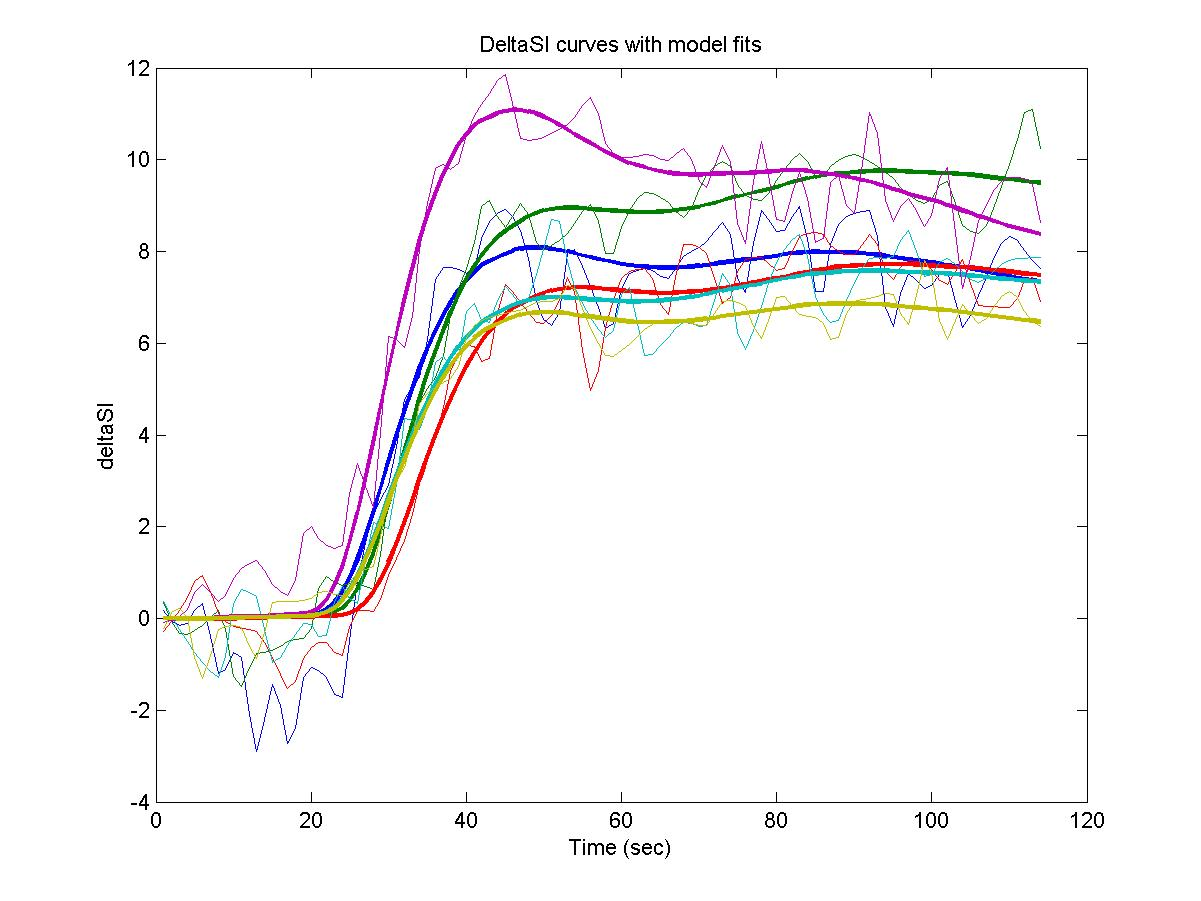
\includegraphics[width=40mm]{Figures/Results_jpg_DZnomask/MoCo_01_DZNoMask_Rest_Fit.jpg} 
    \hspace{-5mm} &
    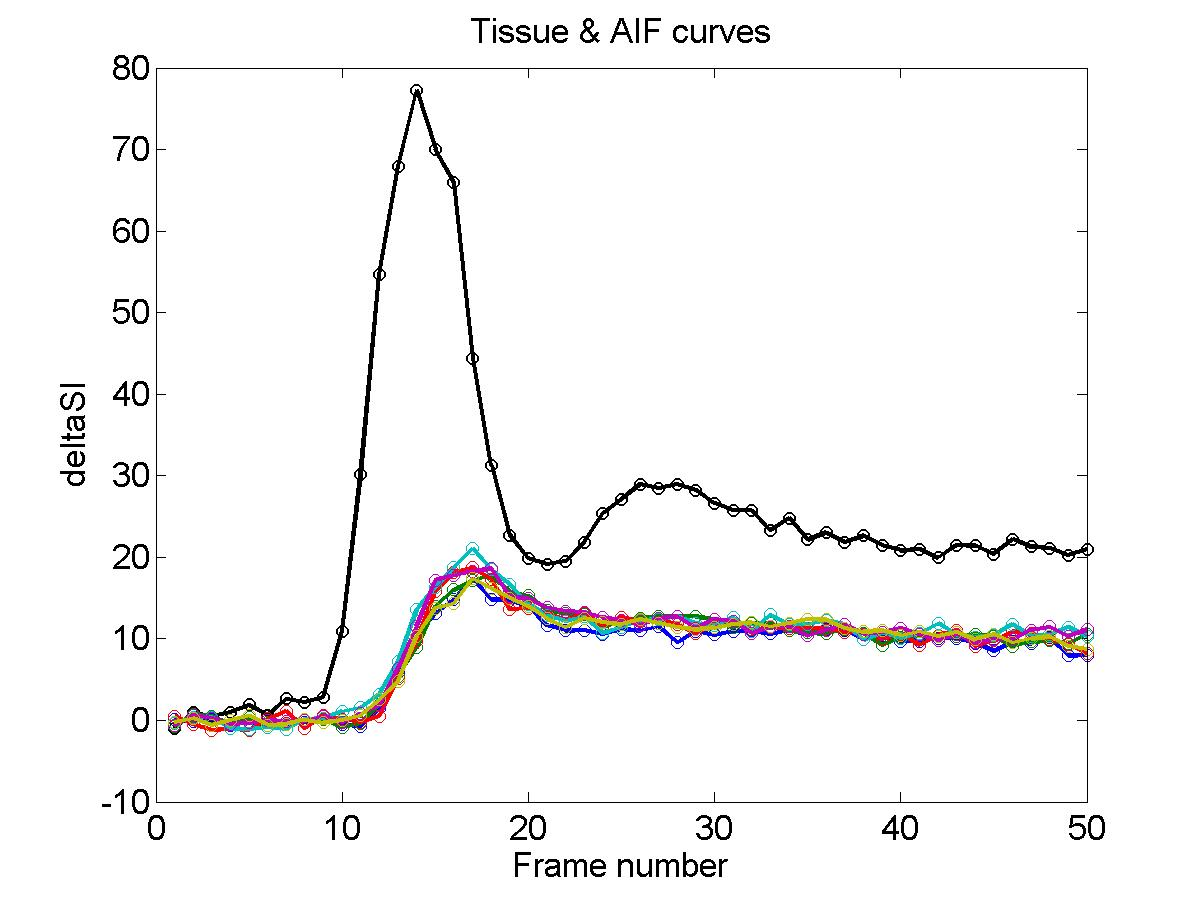
\includegraphics[width=40mm]{Figures/Results_jpg_DZnomask/MoCo_01_DZNoMask_Stress_Curve.jpg} 
    \hspace{-5mm} &
    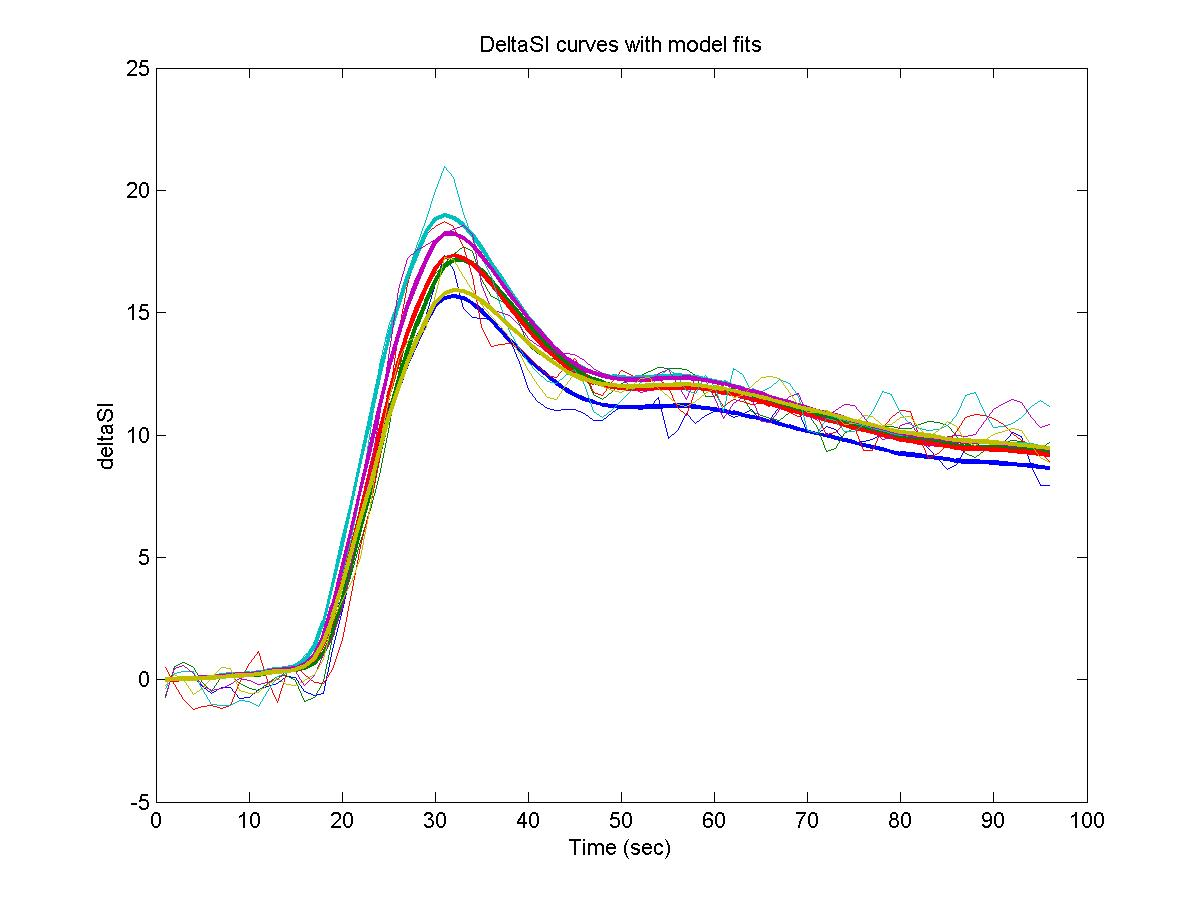
\includegraphics[width=40mm]{Figures/Results_jpg_DZnomask/MoCo_01_DZNoMask_Stress_Fit.jpg} \\
    \rotatebox{90}{\bf \,\,\,\,\,\,\,\,\,\,\,\,\,MoCo\_02} & 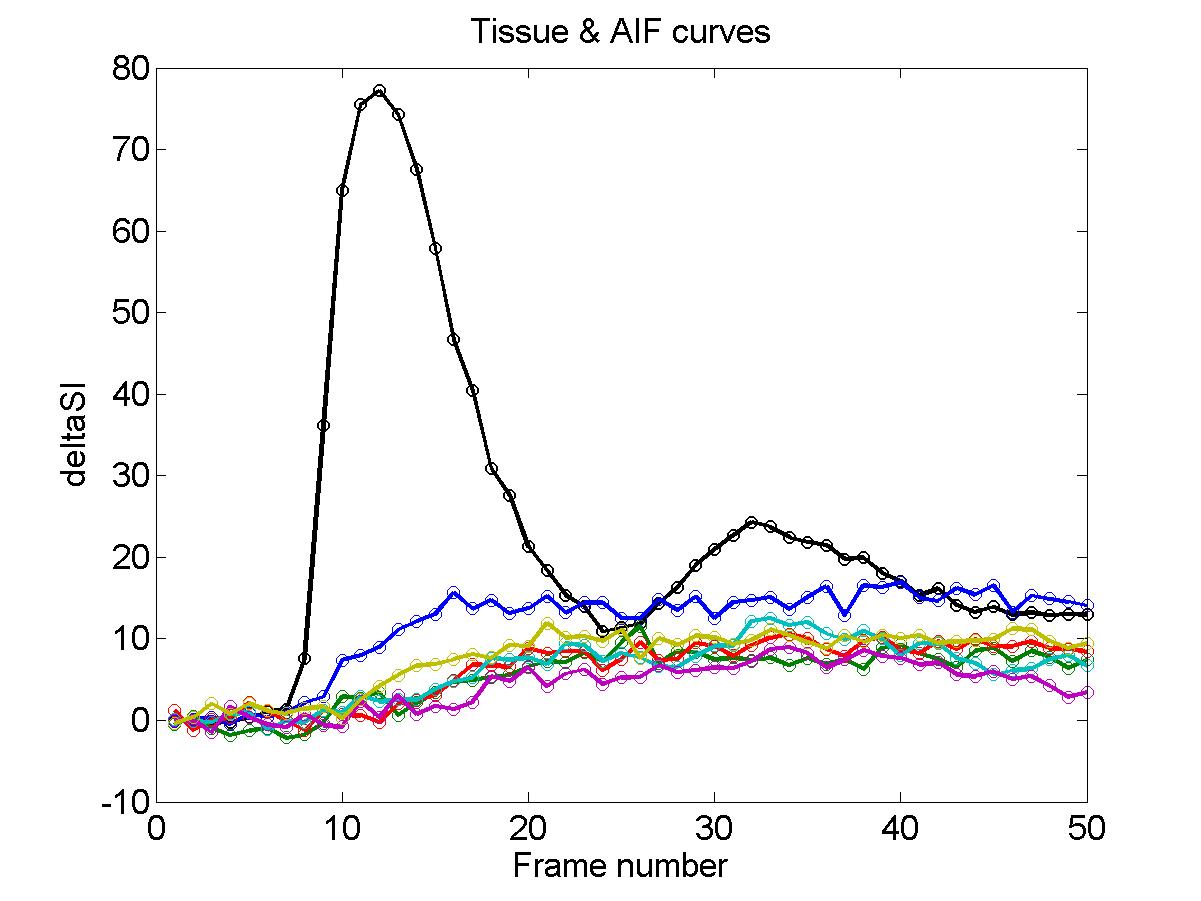
\includegraphics[width=40mm]{Figures/Results_jpg_DZnomask/MoCo_02_DZNoMask_Rest_Curve.jpg} 
    \hspace{-5mm} &
    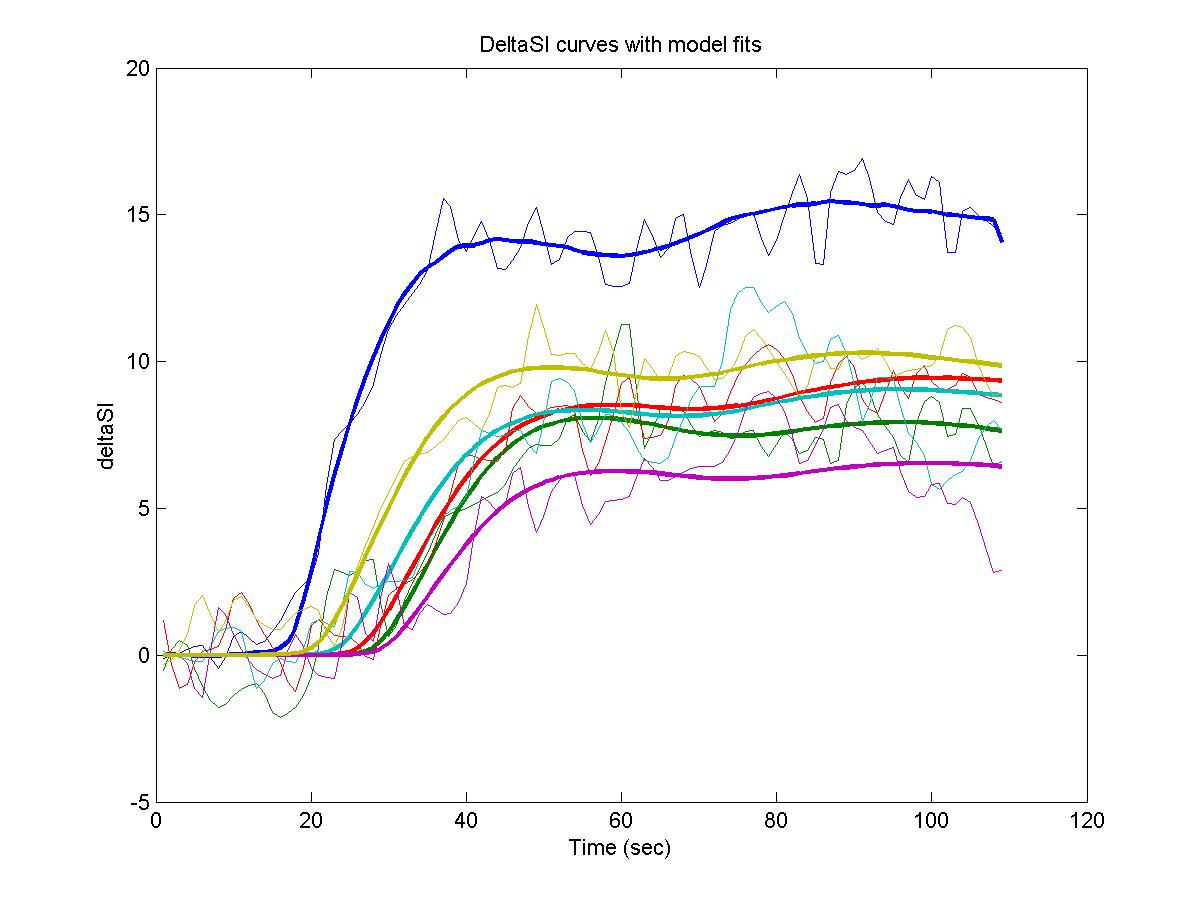
\includegraphics[width=40mm]{Figures/Results_jpg_DZnomask/MoCo_02_DZNoMask_Rest_Fit.jpg} 
    \hspace{-5mm} &
    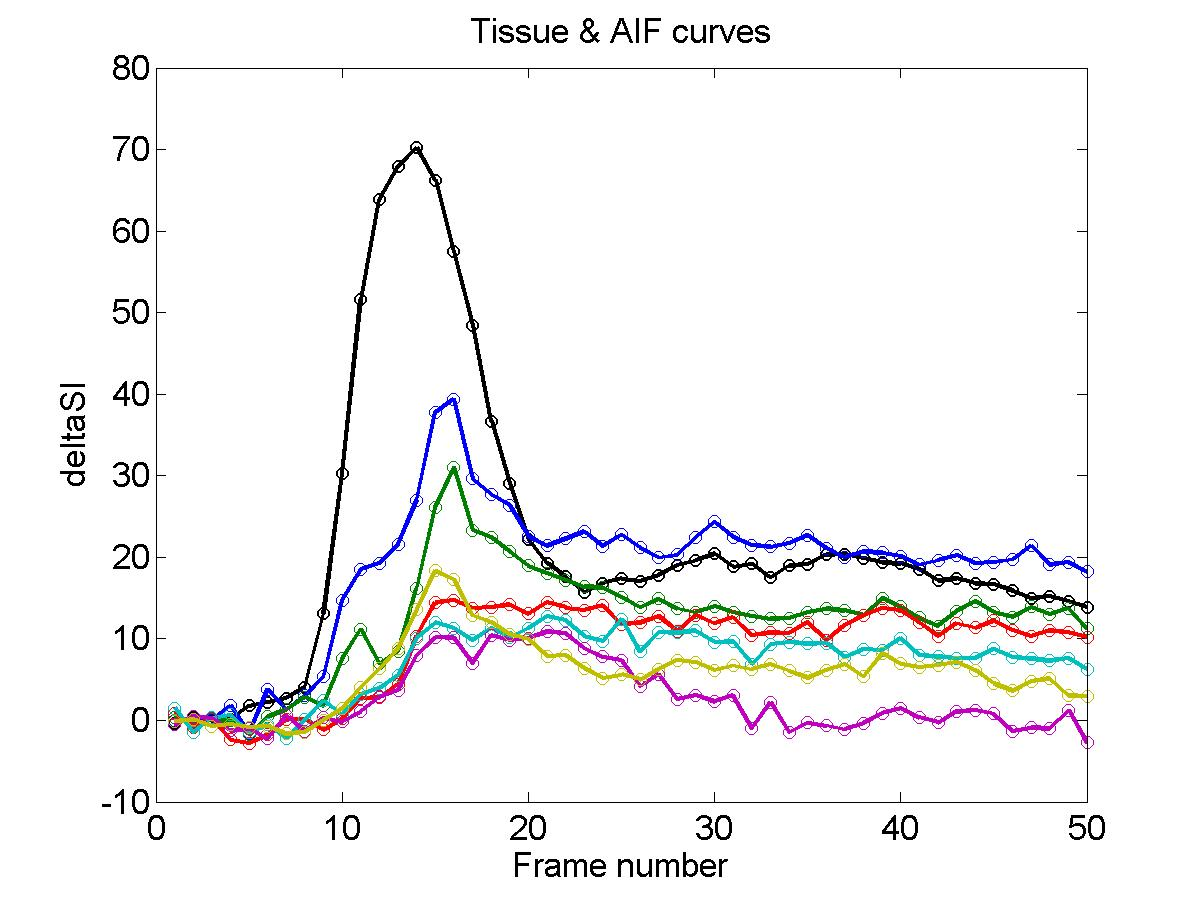
\includegraphics[width=40mm]{Figures/Results_jpg_DZnomask/MoCo_02_DZNoMask_Stress_Curve.jpg} 
    \hspace{-5mm} &
    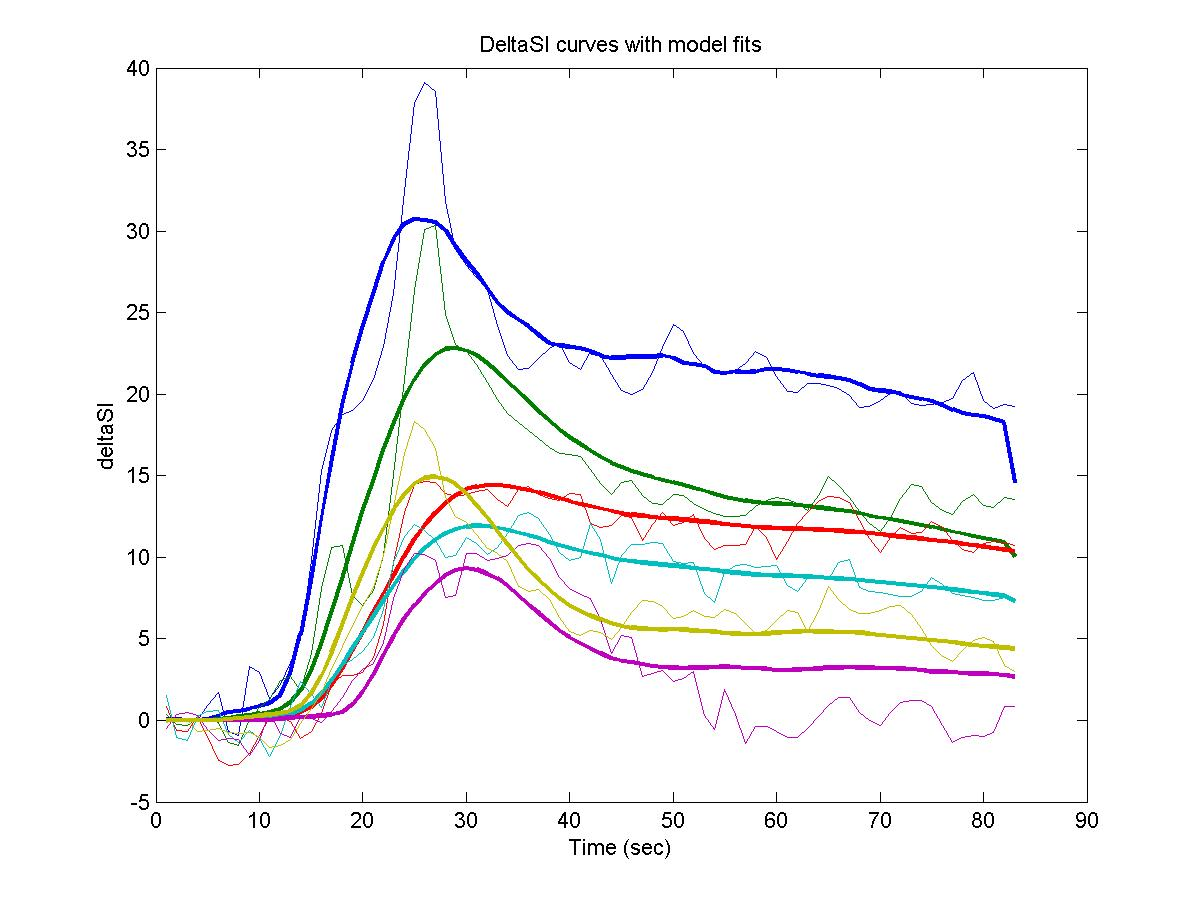
\includegraphics[width=40mm]{Figures/Results_jpg_DZnomask/MoCo_02_DZNoMask_Stress_Fit.jpg} \\
    \rotatebox{90}{\bf \,\,\,\,\,\,\,\,\,\,\,\,\,MoCo\_03} & 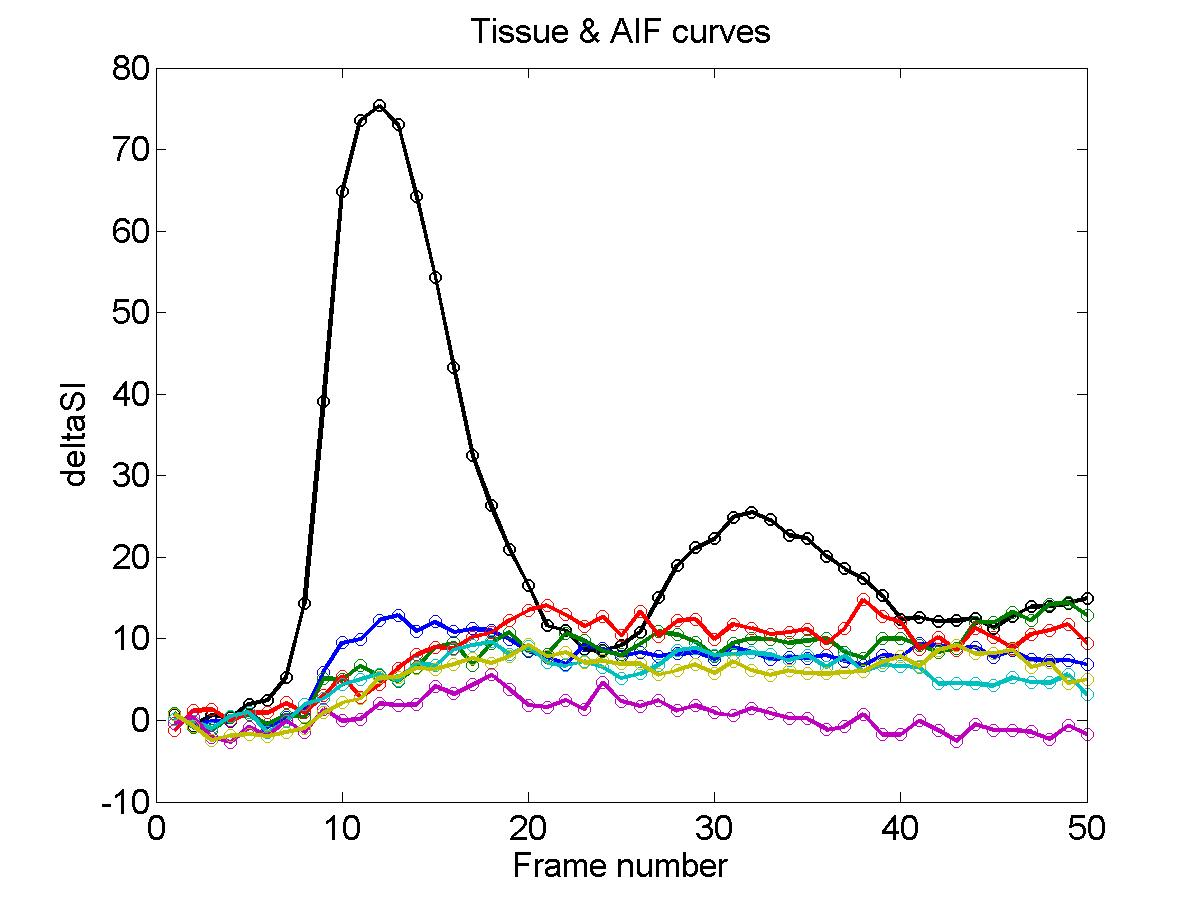
\includegraphics[width=40mm]{Figures/Results_jpg_DZnomask/MoCo_03_DZNoMask_Rest_Curve.jpg} 
    \hspace{-5mm} &
    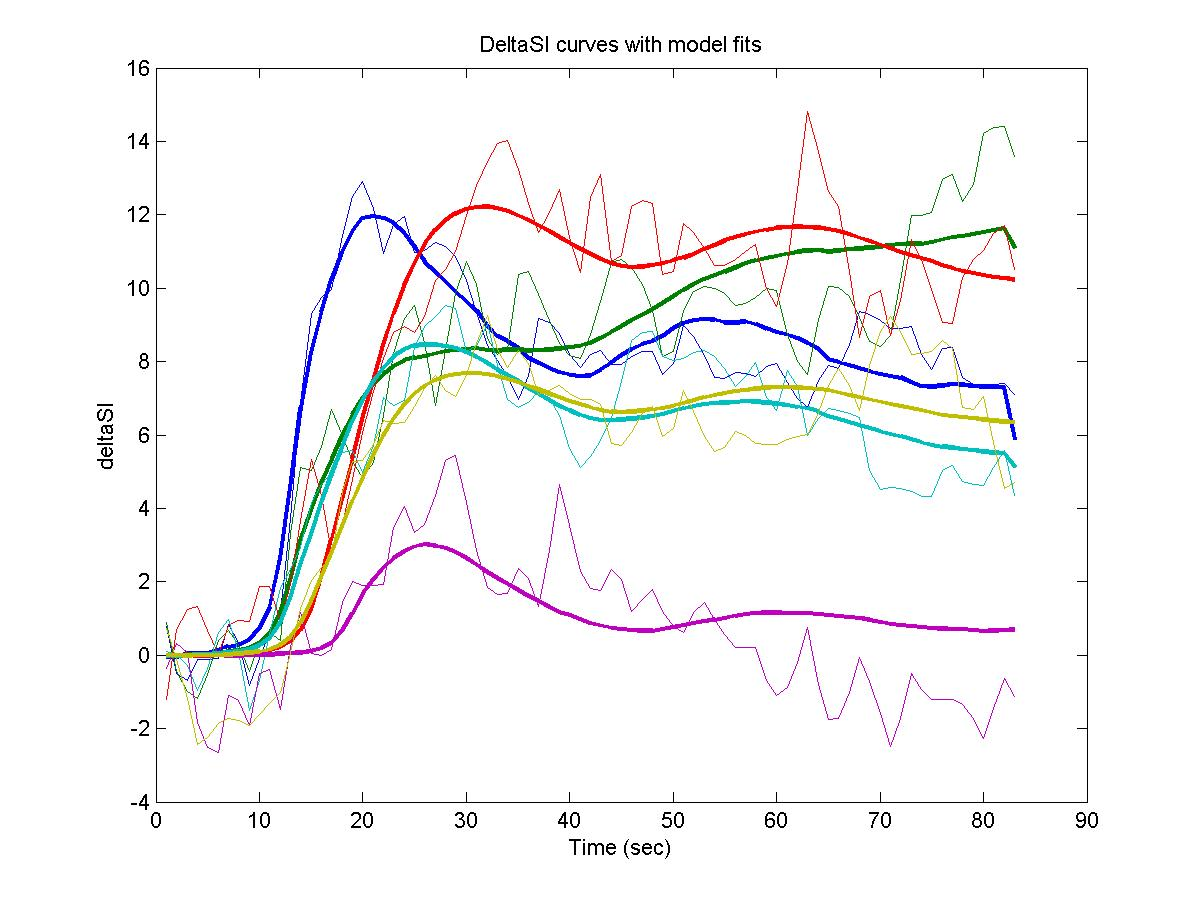
\includegraphics[width=40mm]{Figures/Results_jpg_DZnomask/MoCo_03_DZNoMask_Rest_Fit.jpg} 
    \hspace{-5mm} &
    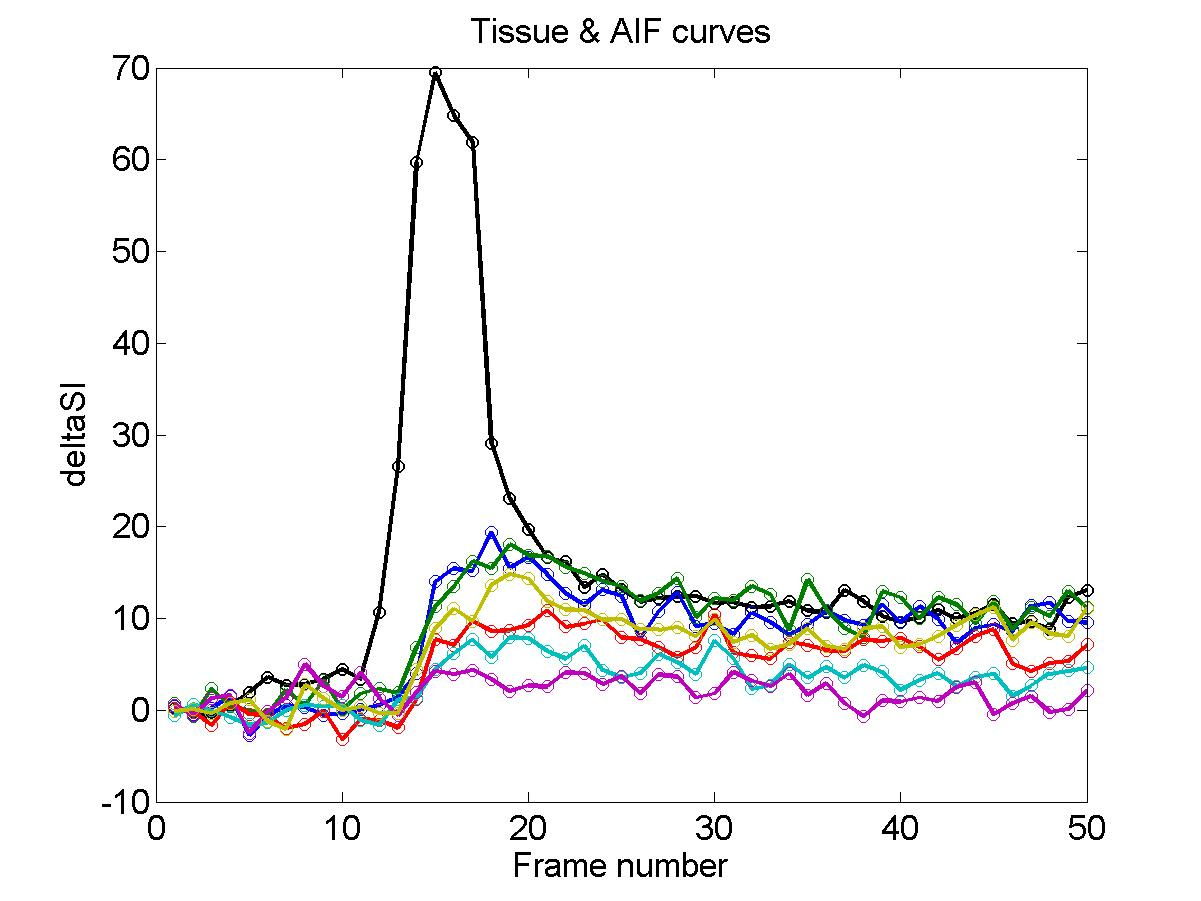
\includegraphics[width=40mm]{Figures/Results_jpg_DZnomask/MoCo_03_DZNoMask_Stress_Curve.jpg} 
    \hspace{-5mm} &
    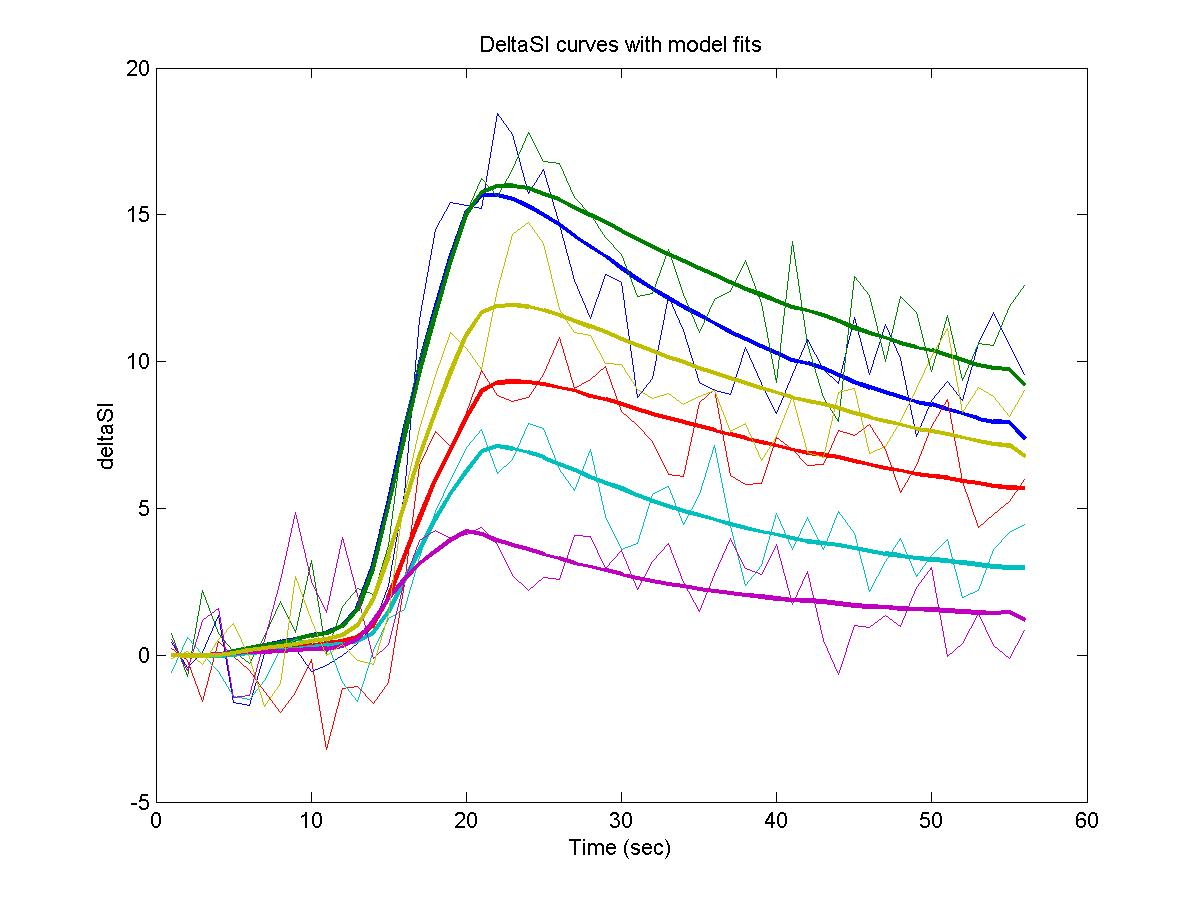
\includegraphics[width=40mm]{Figures/Results_jpg_DZnomask/MoCo_03_DZNoMask_Stress_Fit.jpg} \\
    \rotatebox{90}{\bf \,\,\,\,\,\,\,\,\,\,\,\,\,MoCo\_04} & 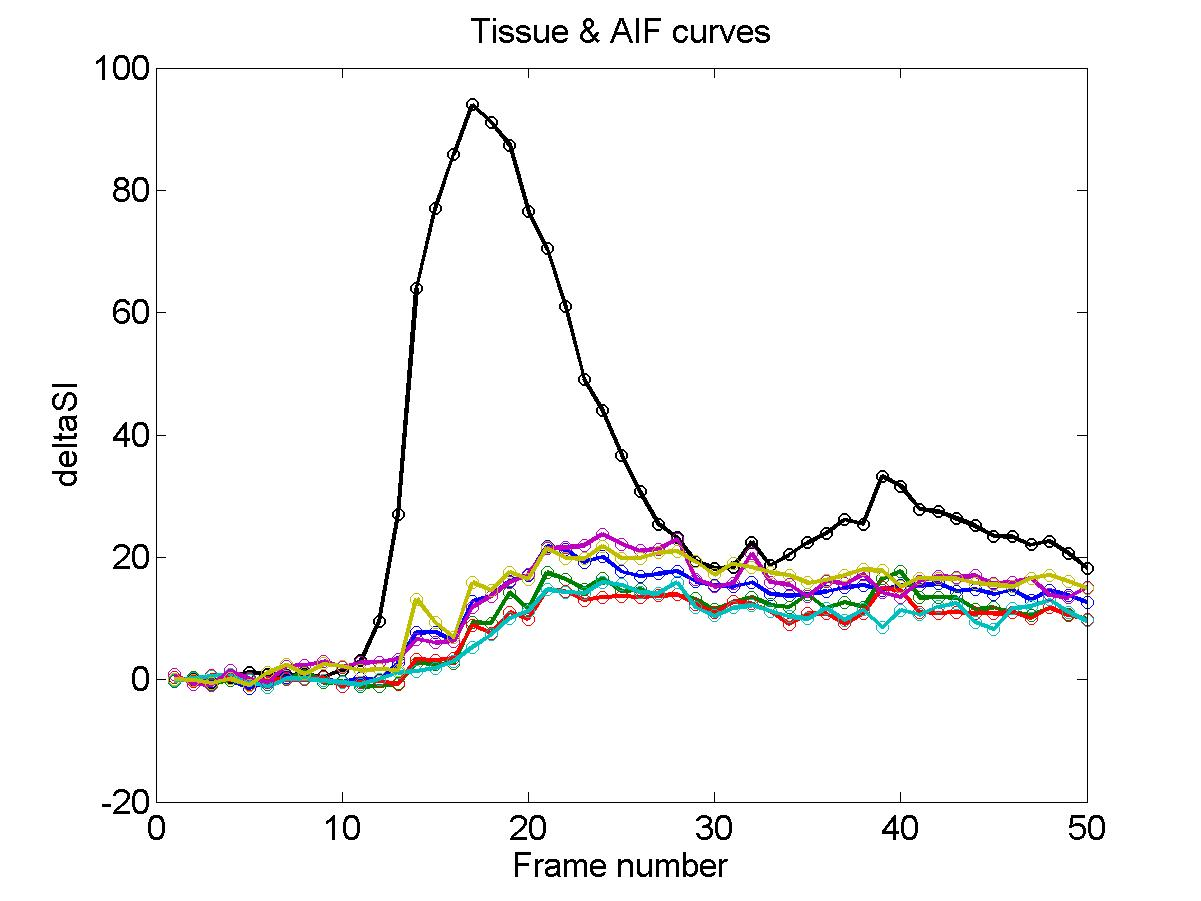
\includegraphics[width=40mm]{Figures/Results_jpg_DZnomask/MoCo_04_DZNoMask_Rest_Curve.jpg} 
    \hspace{-5mm} &
    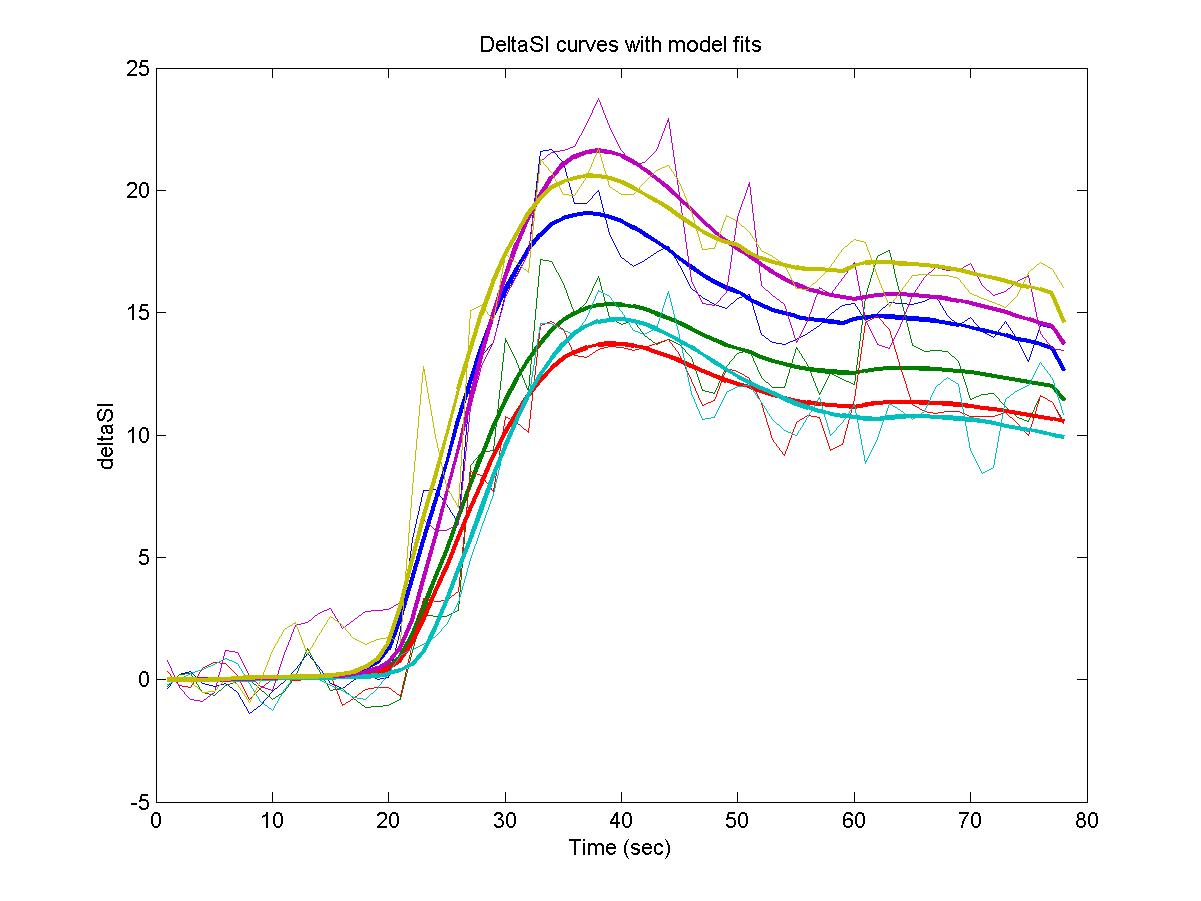
\includegraphics[width=40mm]{Figures/Results_jpg_DZnomask/MoCo_04_DZNoMask_Rest_Fit.jpg} 
    \hspace{-5mm} &
    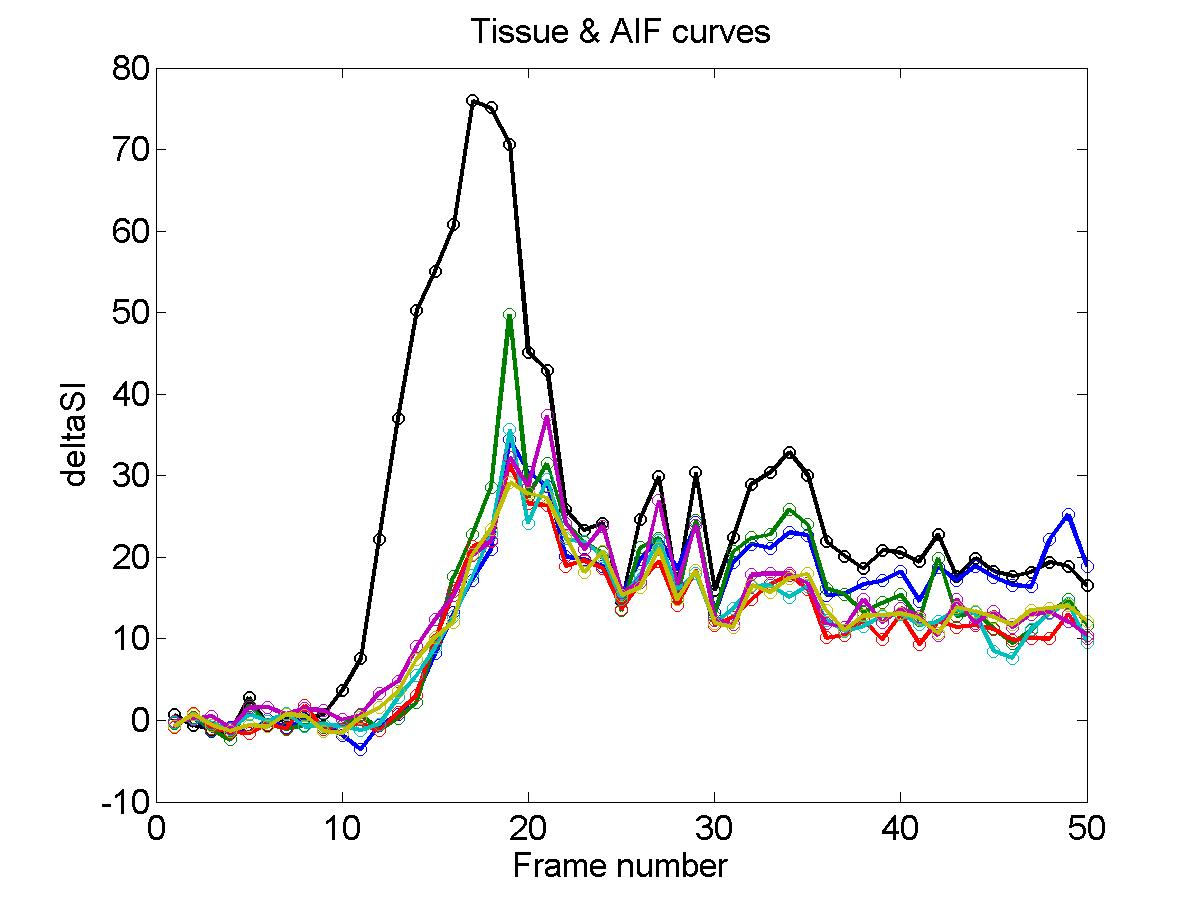
\includegraphics[width=40mm]{Figures/Results_jpg_DZnomask/MoCo_04_DZNoMask_Stress_Curve.jpg} 
    \hspace{-5mm} &
    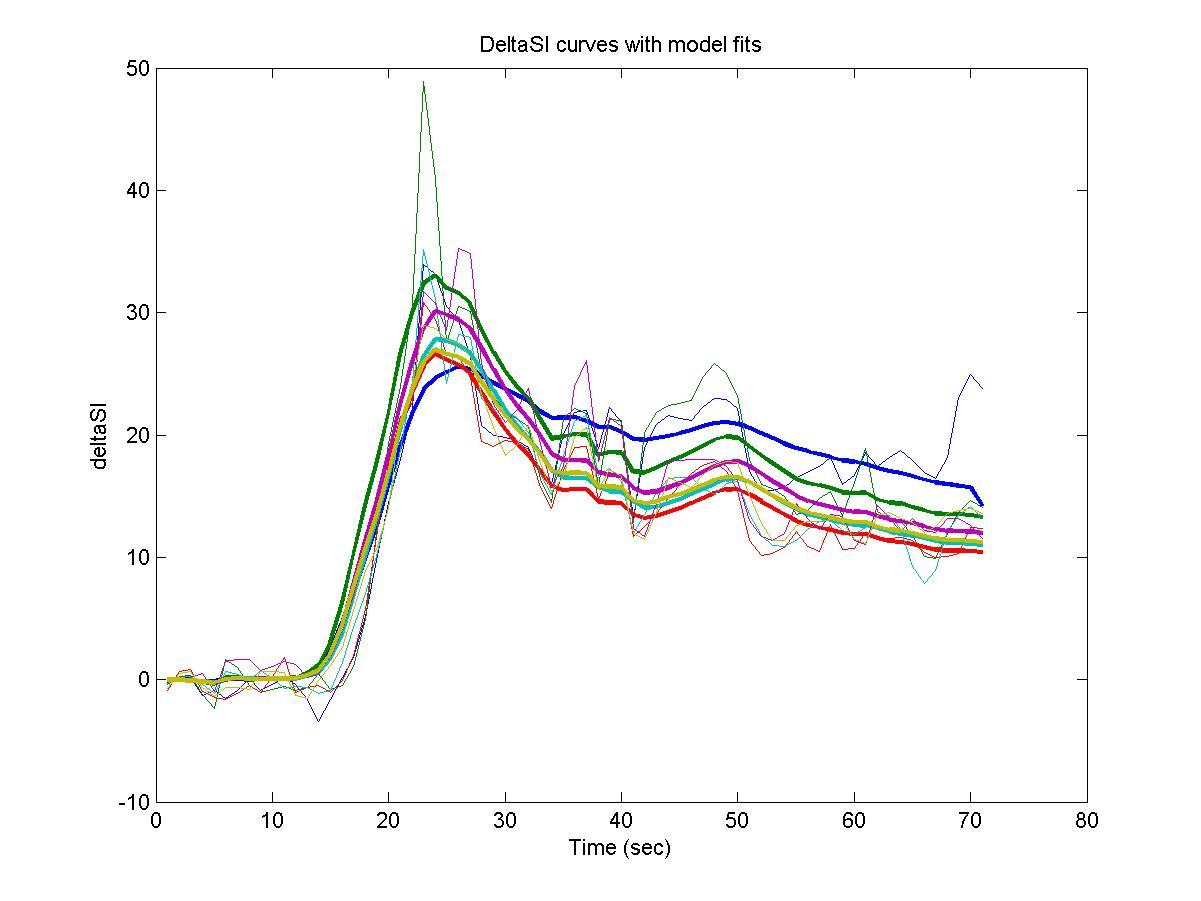
\includegraphics[width=40mm]{Figures/Results_jpg_DZnomask/MoCo_04_DZNoMask_Stress_Fit.jpg} \\
    \rotatebox{90}{\bf \,\,\,\,\,\,\,\,\,\,\,\,\,MoCo\_05} & 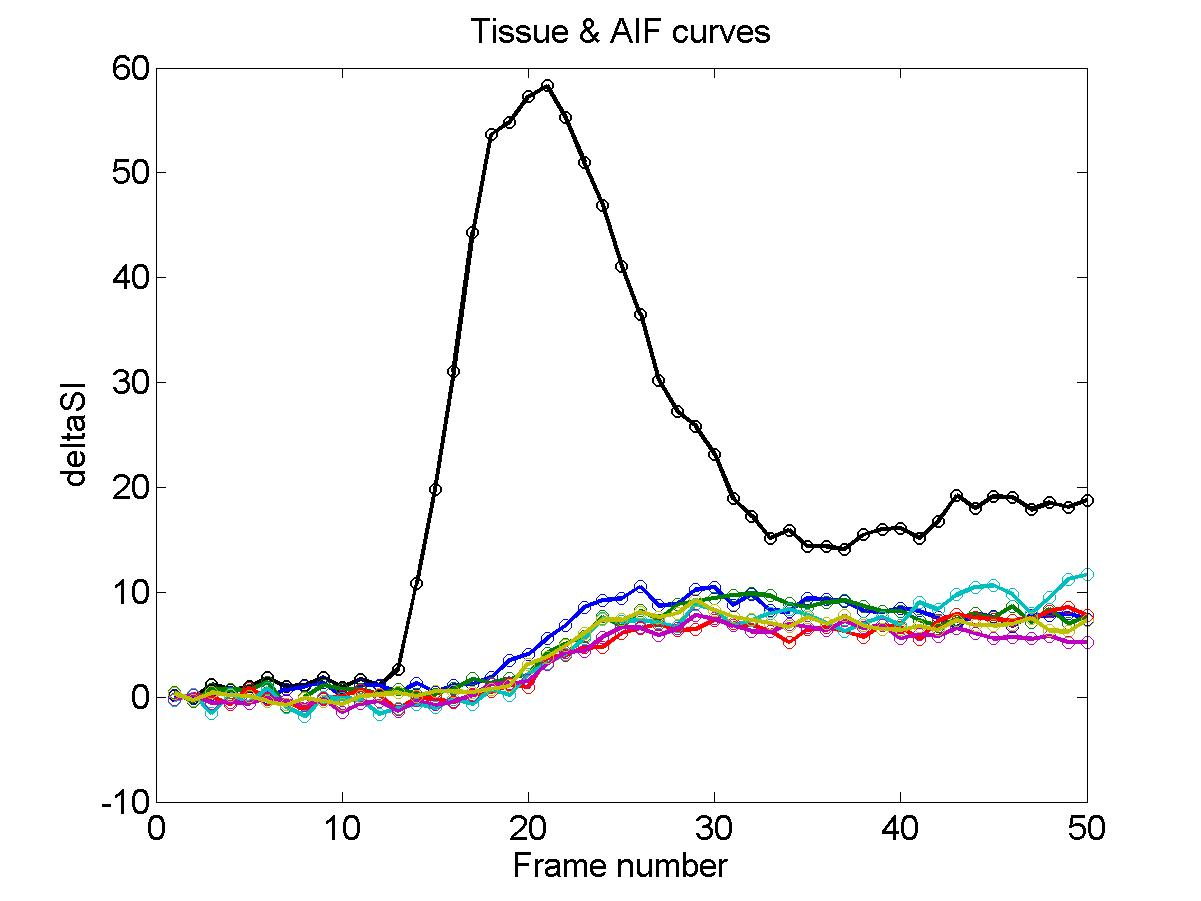
\includegraphics[width=40mm]{Figures/Results_jpg_DZnomask/MoCo_05_DZNoMask_Rest_Curve.jpg} 
    \hspace{-5mm} &
    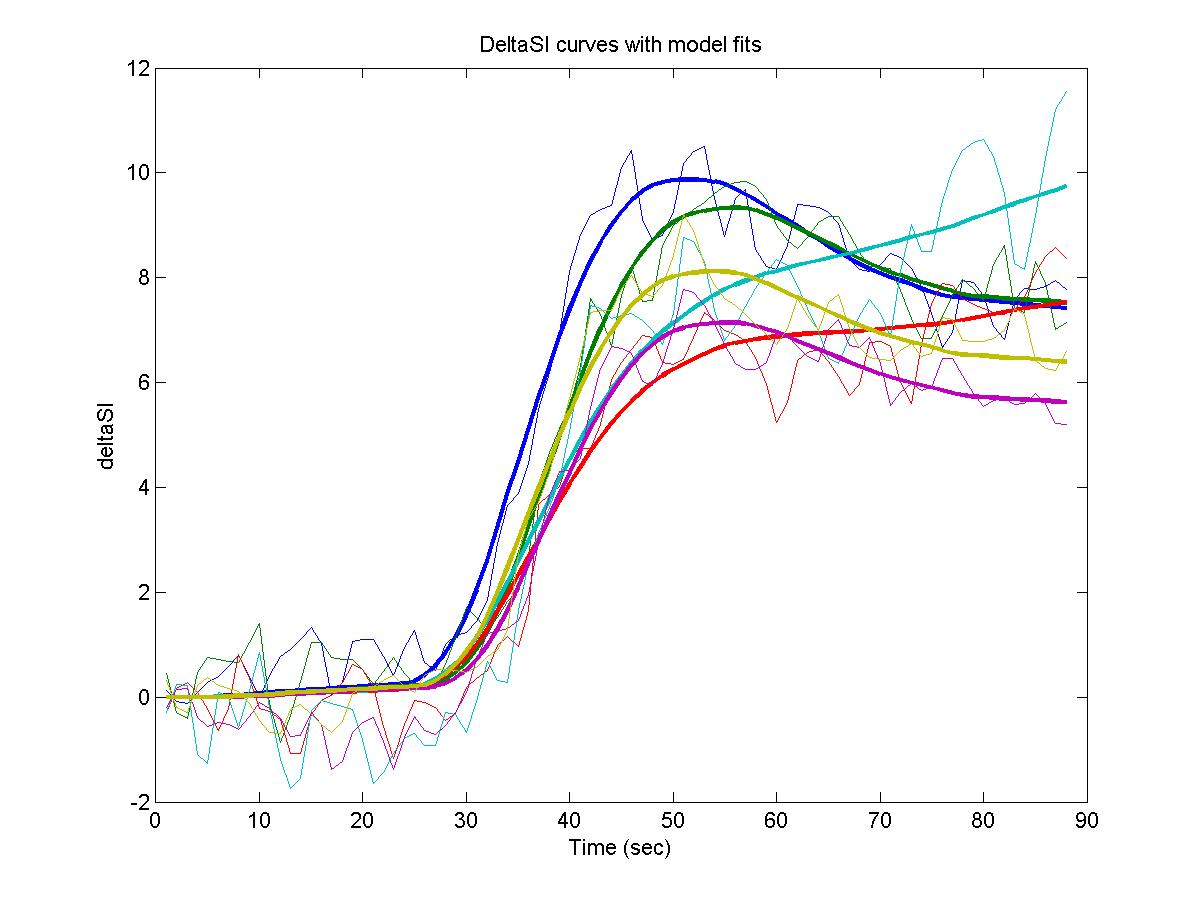
\includegraphics[width=40mm]{Figures/Results_jpg_DZnomask/MoCo_05_DZNoMask_Rest_Fit.jpg} 
    \hspace{-5mm} &
    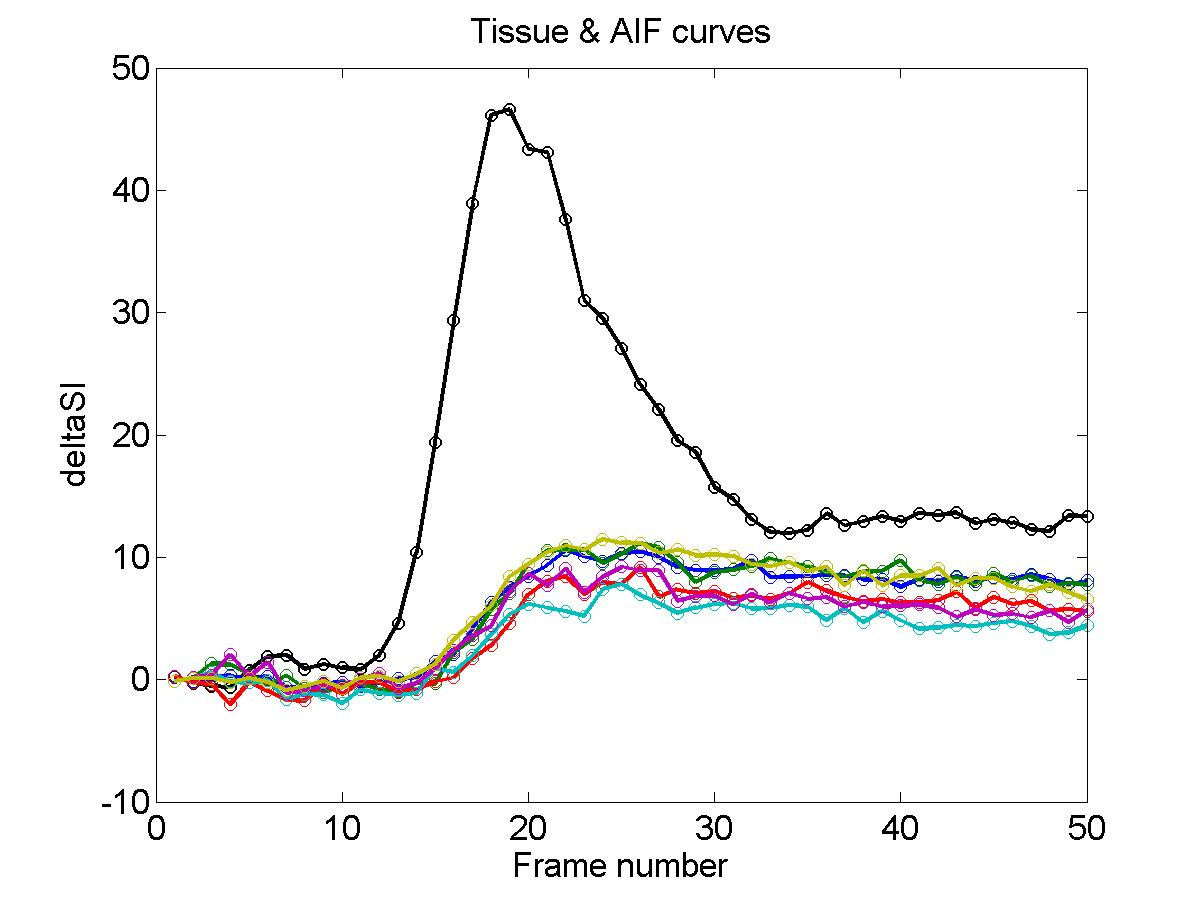
\includegraphics[width=40mm]{Figures/Results_jpg_DZnomask/MoCo_05_DZNoMask_Stress_Curve.jpg} 
    \hspace{-5mm} &
    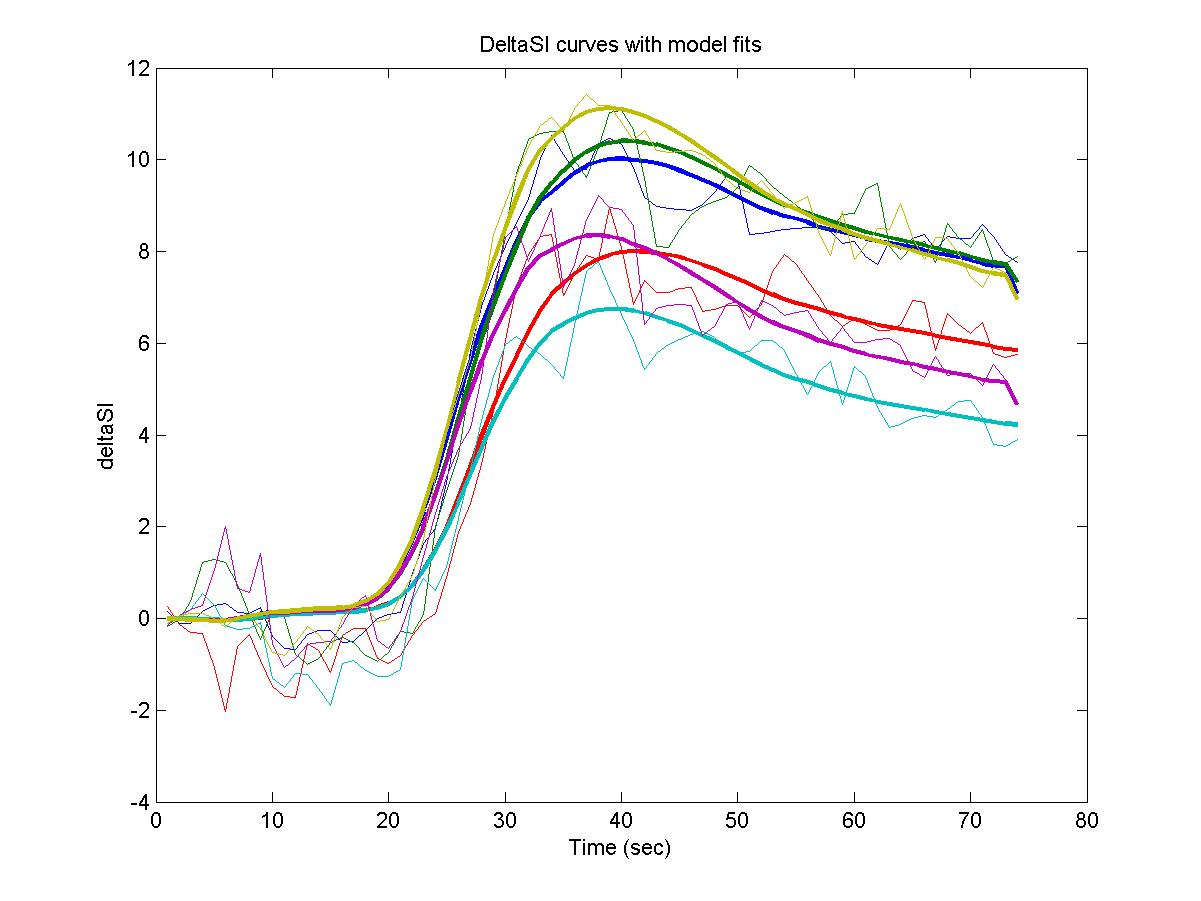
\includegraphics[width=40mm]{Figures/Results_jpg_DZnomask/MoCo_05_DZNoMask_Stress_Fit.jpg} \\
  \end{tabular}
  }
  \caption{Validation time curves consisting of tissue and arterial input function time plots 
  for the first five gated data sets.}
  \label{fig:gated1}
\end{figure}

\begin{figure}
 \makebox[\textwidth][c]{
   \begin{tabular}{ccccc}
    {} & \multicolumn{2}{c}{\bf Rest} &  \multicolumn{2}{c}{\bf Stress} \\
    \rotatebox{90}{\bf \,\,\,\,\,\,\,\,\,\,\,\,\,MoCo\_06} & 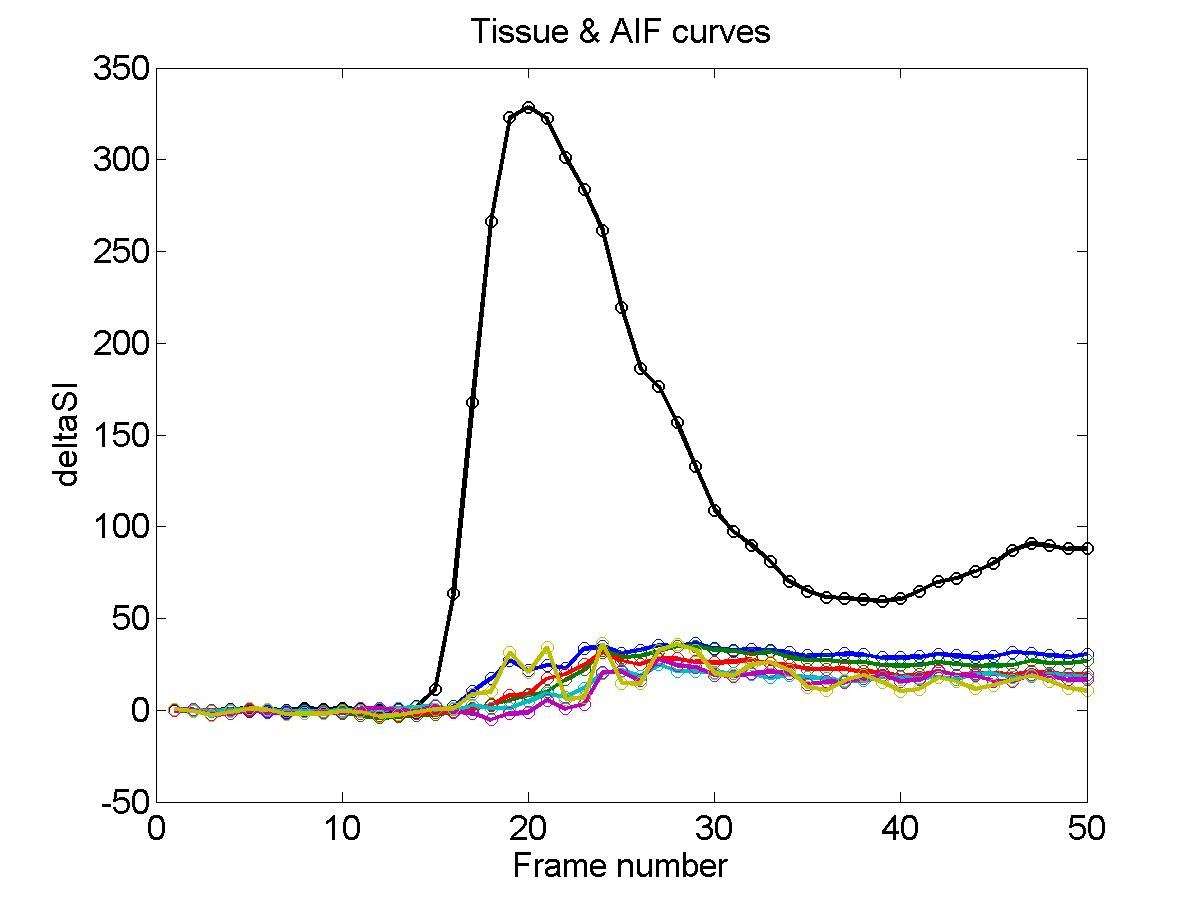
\includegraphics[width=40mm]{Figures/Results_jpg_DZnomask/MoCo_06_DZNoMask_Rest_Curve.jpg} 
    \hspace{-5mm} &
    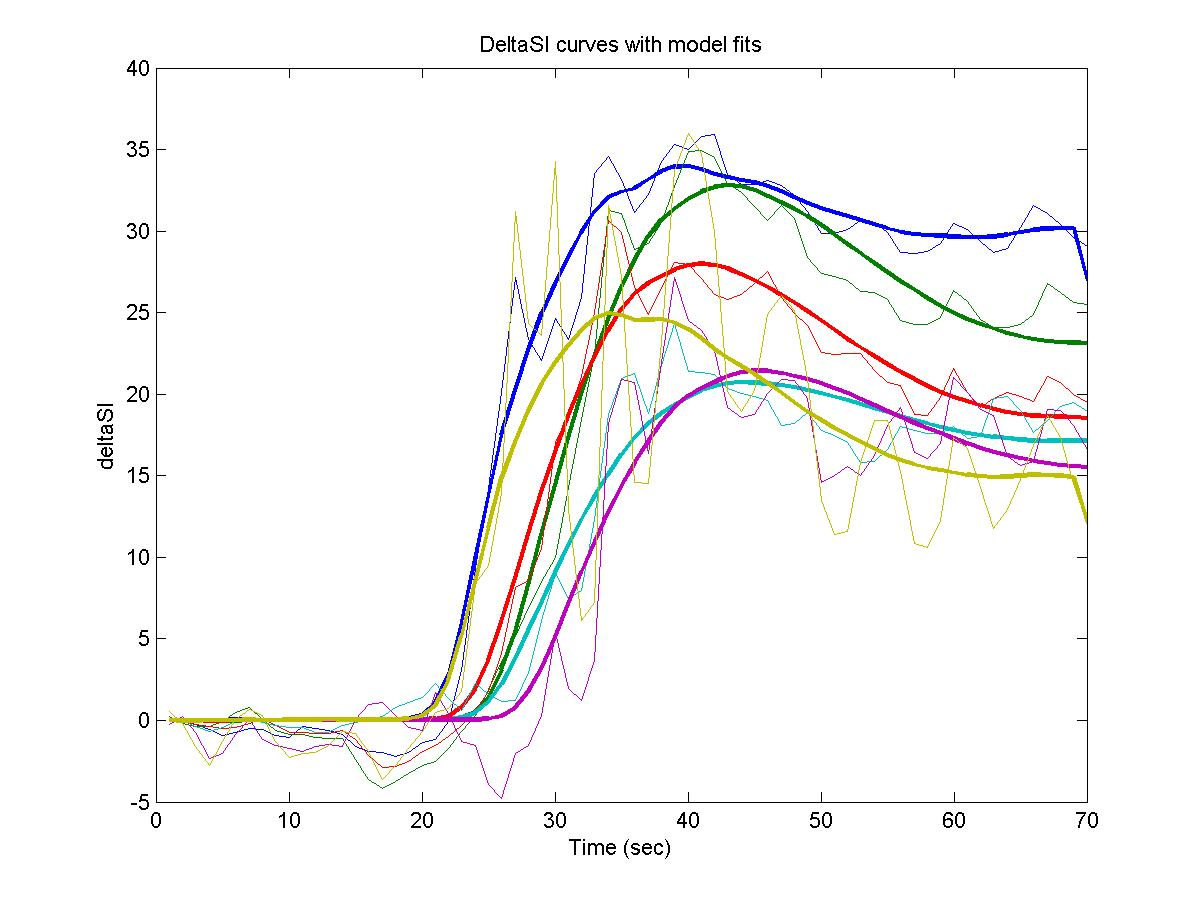
\includegraphics[width=40mm]{Figures/Results_jpg_DZnomask/MoCo_06_DZNoMask_Rest_Fit.jpg} 
    \hspace{-5mm} &
    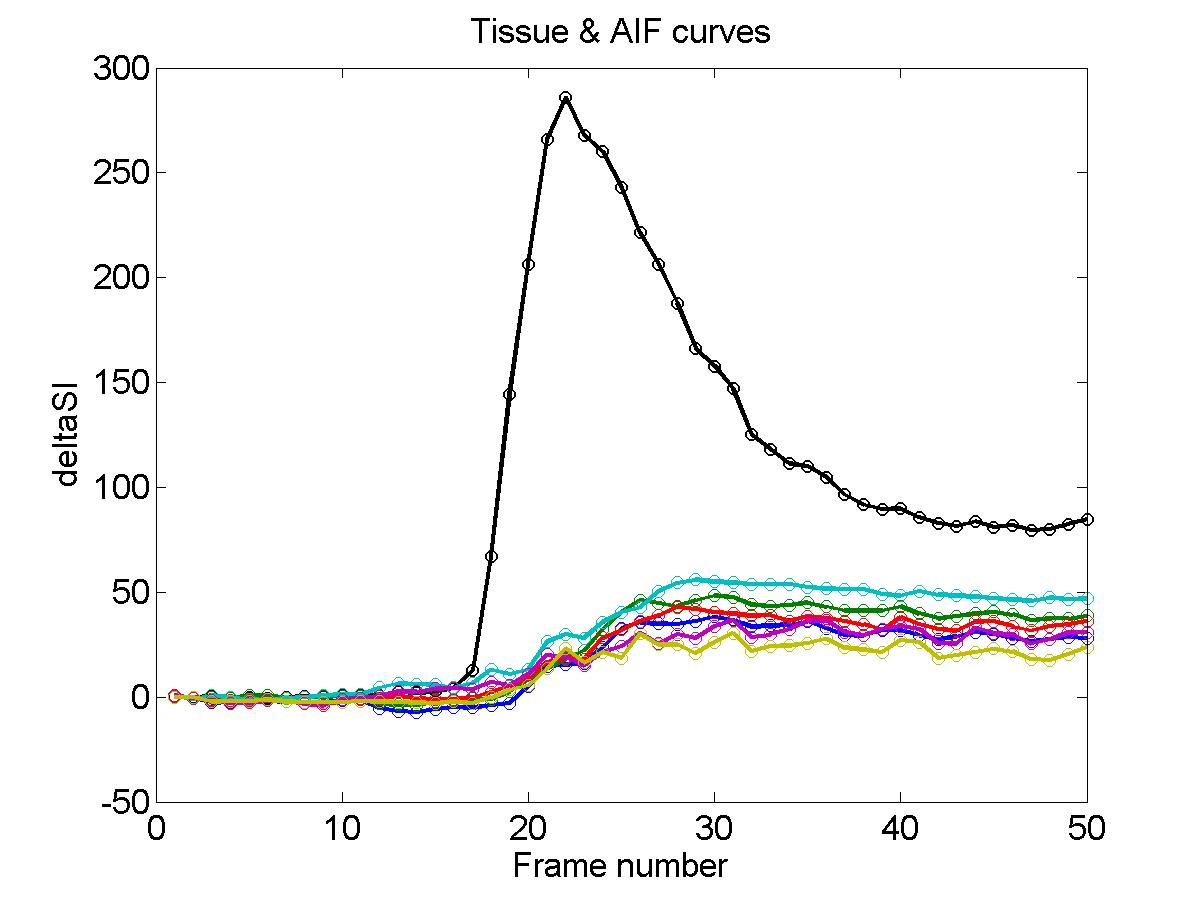
\includegraphics[width=40mm]{Figures/Results_jpg_DZnomask/MoCo_06_DZNoMask_Stress_Curve.jpg} 
    \hspace{-5mm} &
    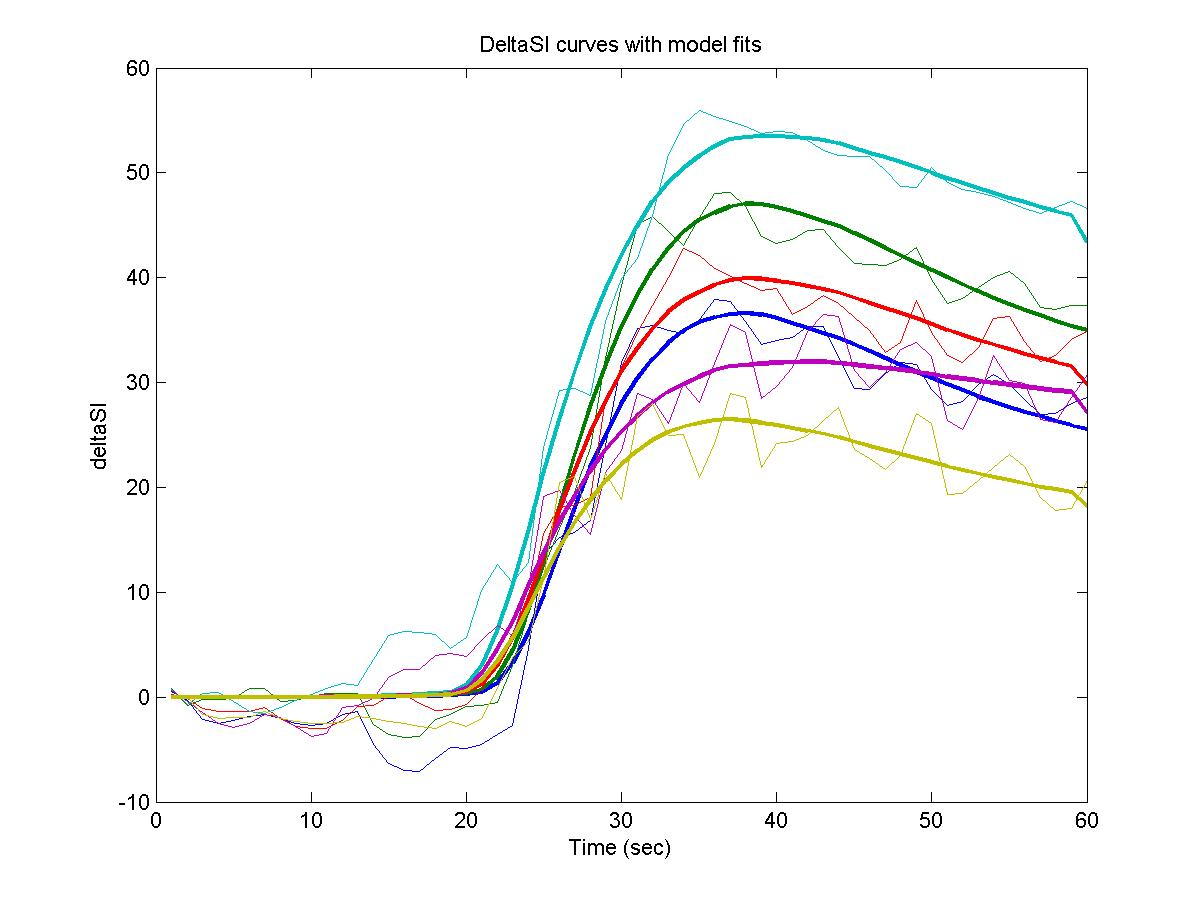
\includegraphics[width=40mm]{Figures/Results_jpg_DZnomask/MoCo_06_DZNoMask_Stress_Fit.jpg} \\
    \rotatebox{90}{\bf \,\,\,\,\,\,\,\,\,\,\,\,\,MoCo\_07} & 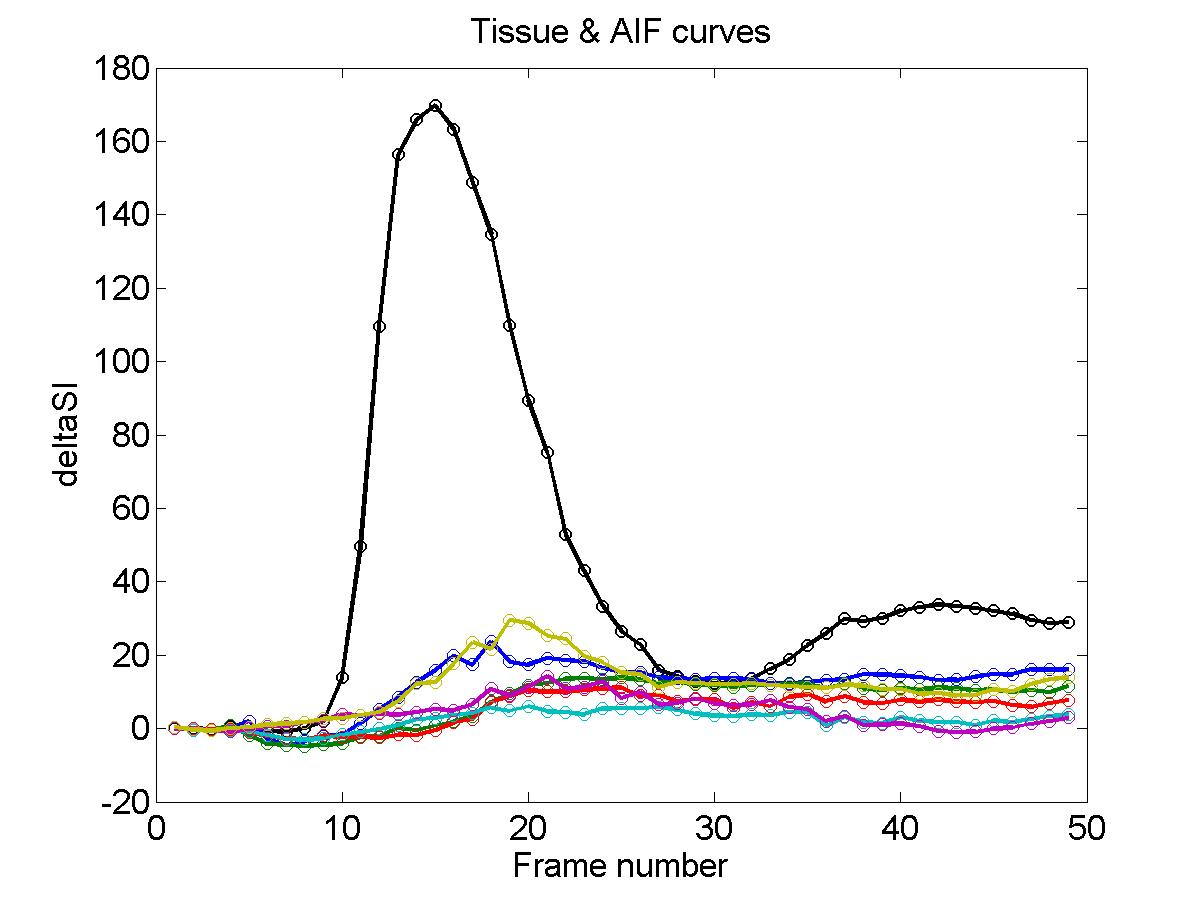
\includegraphics[width=40mm]{Figures/Results_jpg_DZnomask/MoCo_07_DZNoMask_Rest_Curve.jpg} 
    \hspace{-5mm} &
    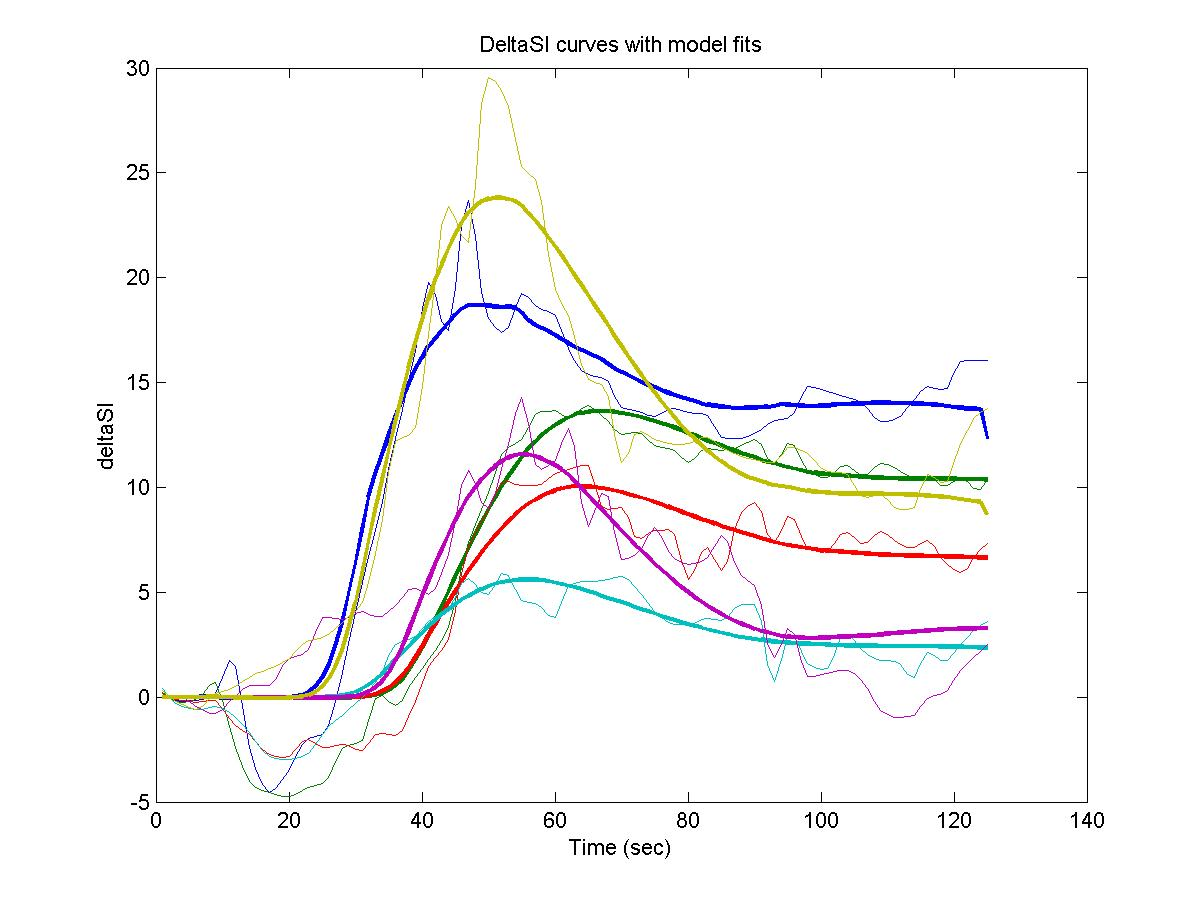
\includegraphics[width=40mm]{Figures/Results_jpg_DZnomask/MoCo_07_DZNoMask_Rest_Fit.jpg} 
    \hspace{-5mm} &
    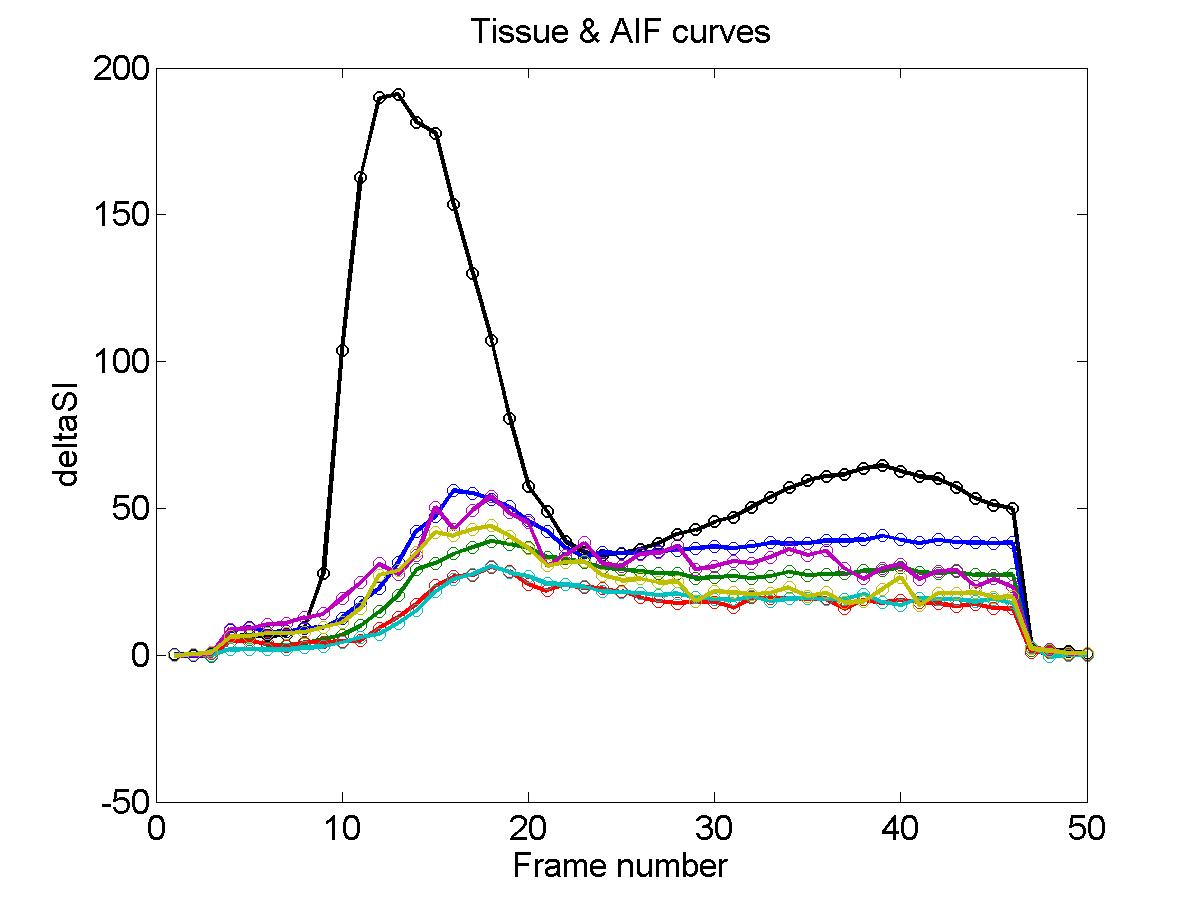
\includegraphics[width=40mm]{Figures/Results_jpg_DZnomask/MoCo_07_DZNoMask_Stress_Curve.jpg} 
    \hspace{-5mm} &
    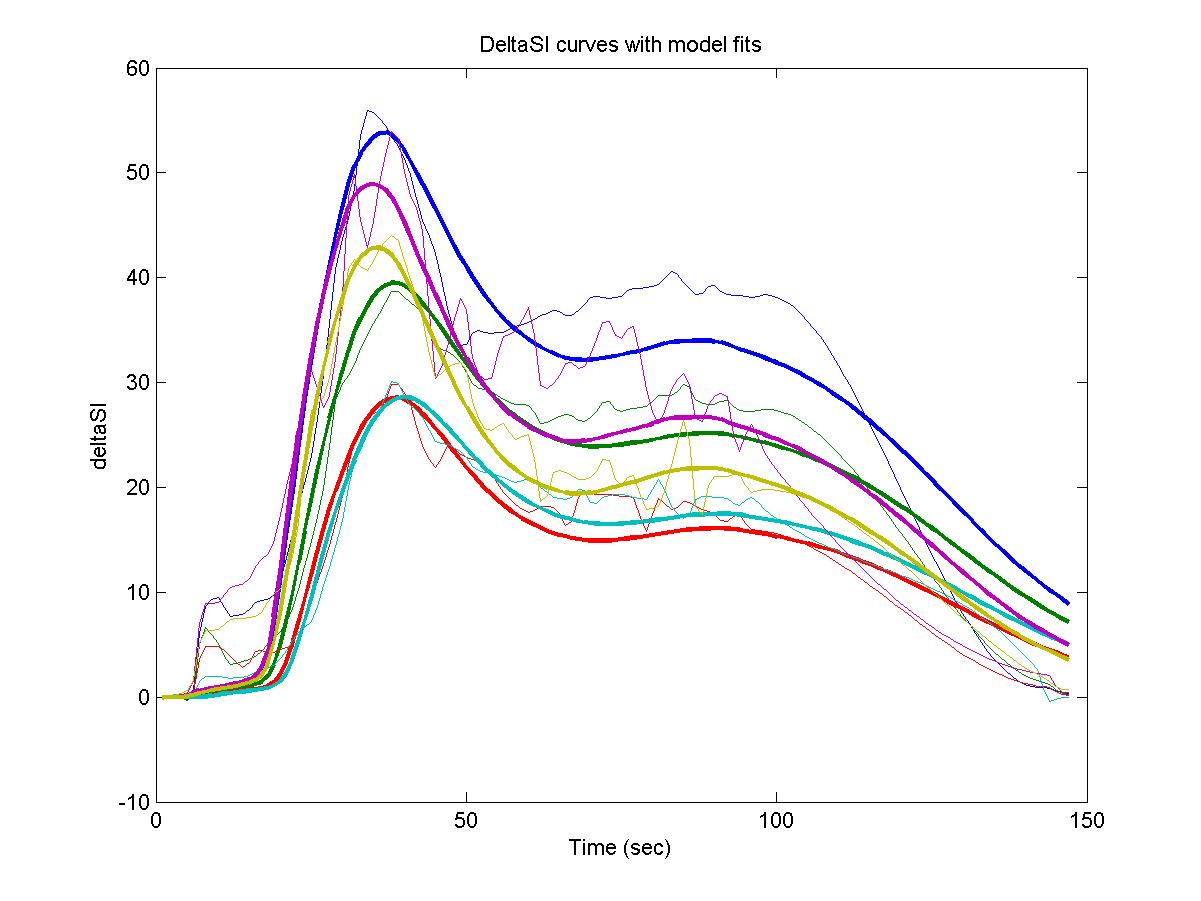
\includegraphics[width=40mm]{Figures/Results_jpg_DZnomask/MoCo_07_DZNoMask_Stress_Fit.jpg} \\
    \rotatebox{90}{\bf \,\,\,\,\,\,\,\,\,\,\,\,\,MoCo\_08} & 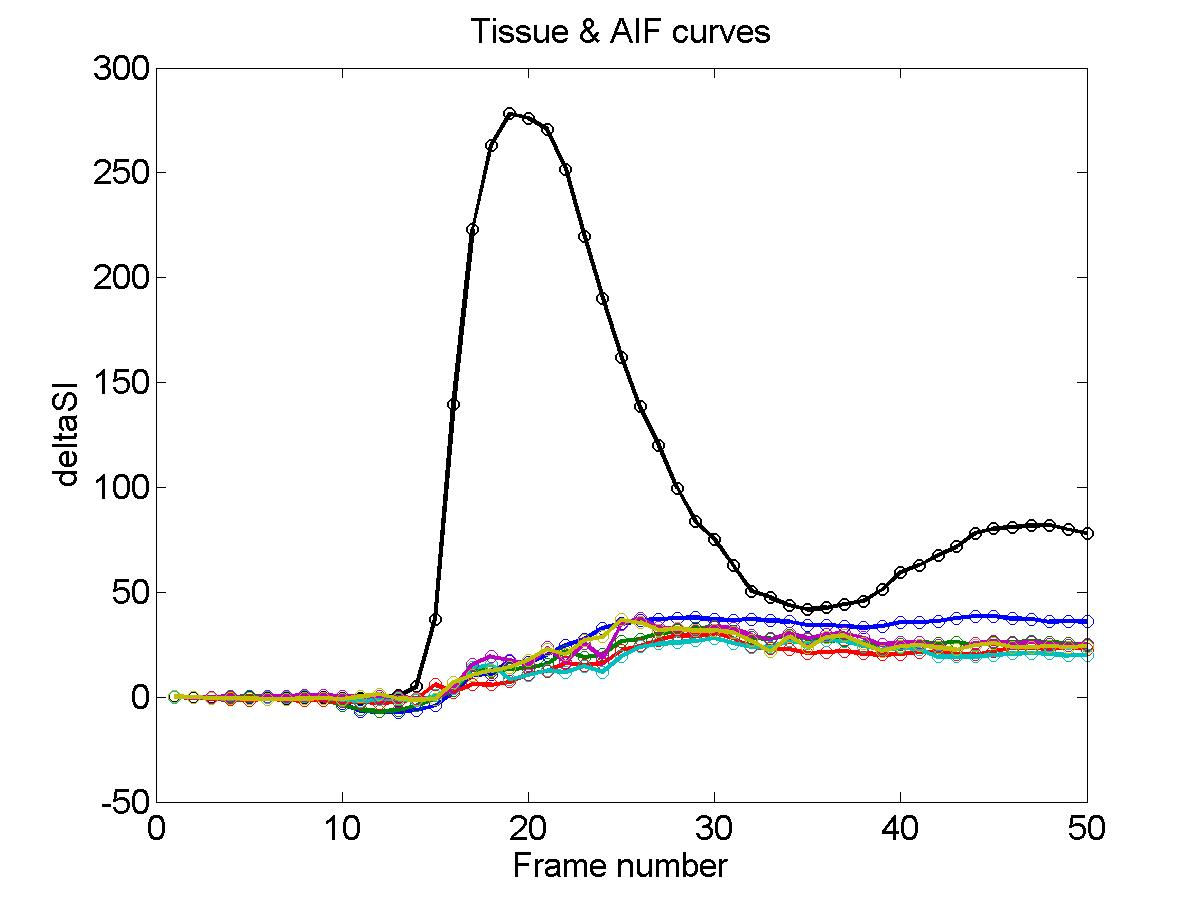
\includegraphics[width=40mm]{Figures/Results_jpg_DZnomask/MoCo_08_DZNoMask_Rest_Curve.jpg} 
    \hspace{-5mm} &
    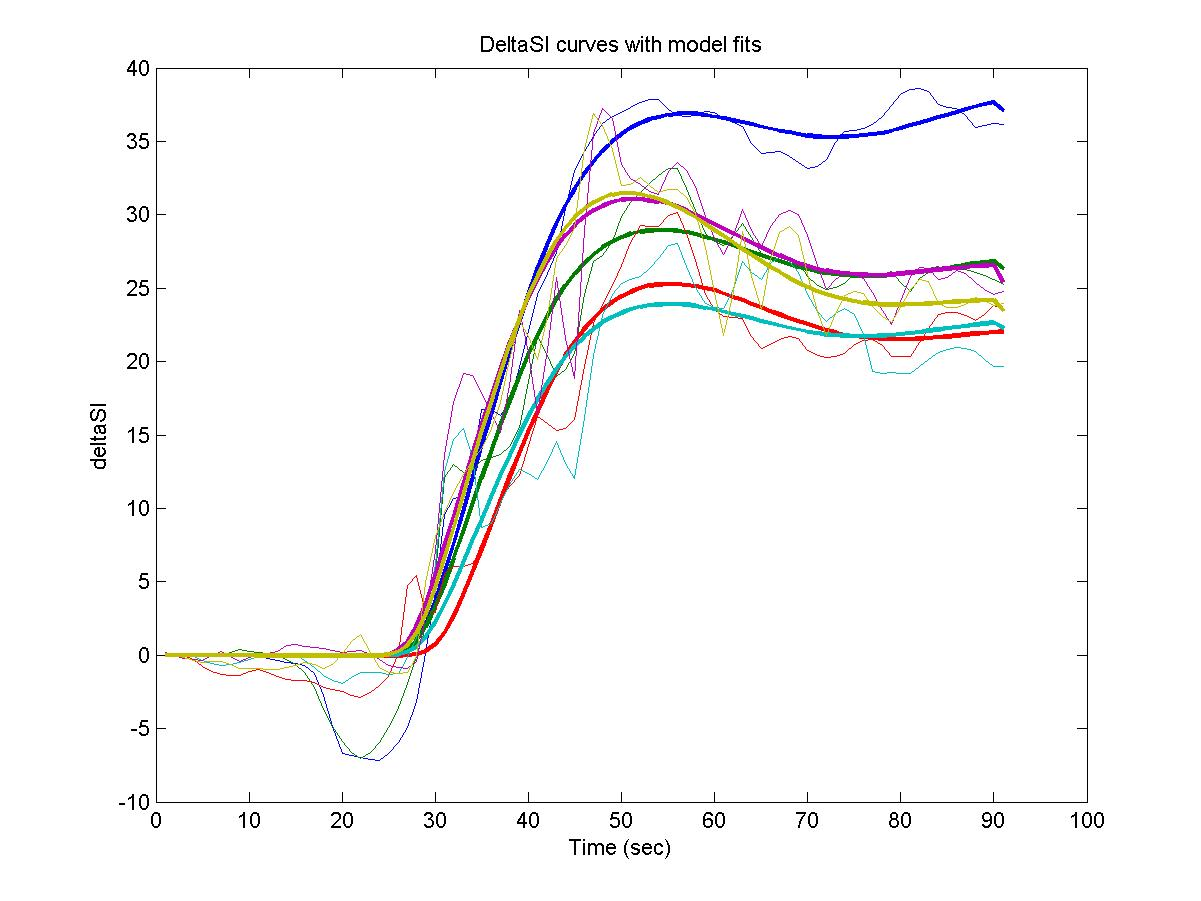
\includegraphics[width=40mm]{Figures/Results_jpg_DZnomask/MoCo_08_DZNoMask_Rest_Fit.jpg} 
    \hspace{-5mm} &
    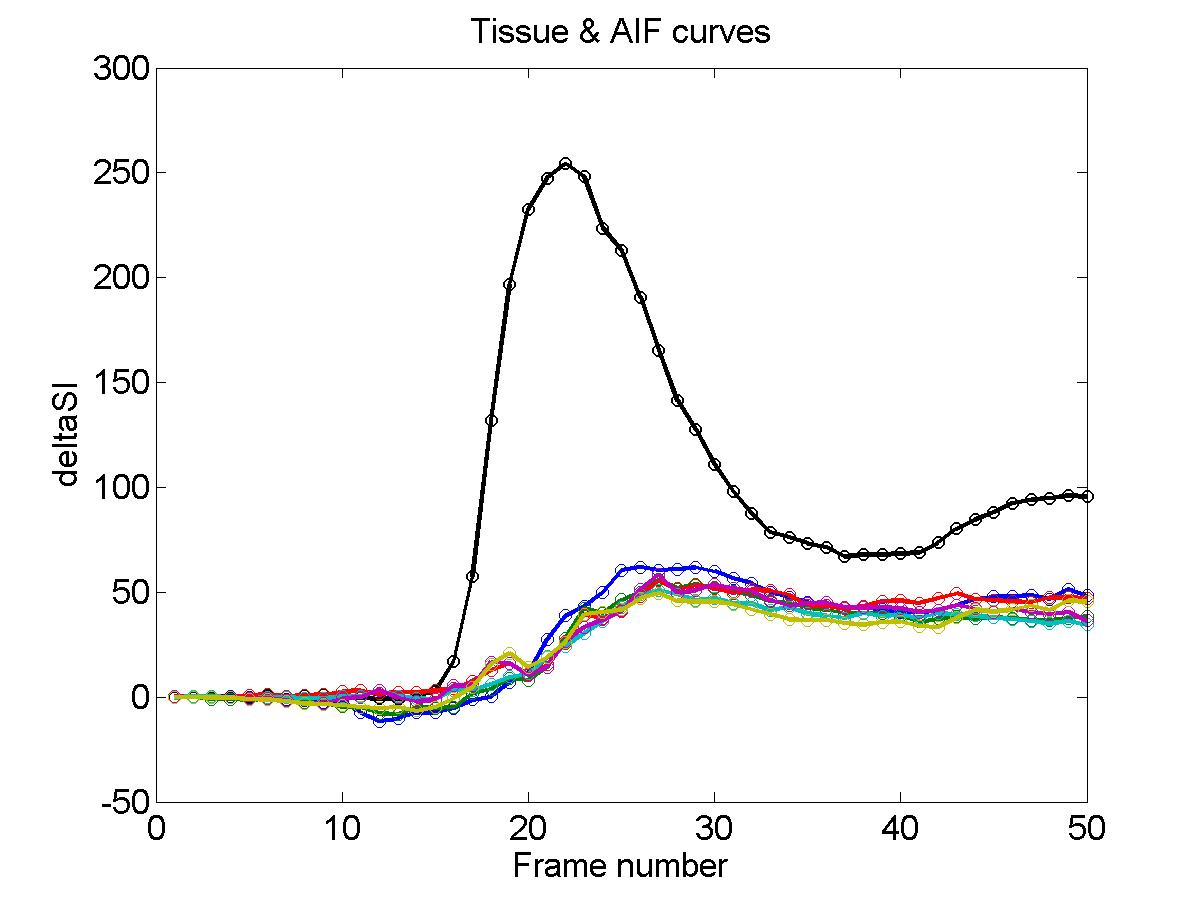
\includegraphics[width=40mm]{Figures/Results_jpg_DZnomask/MoCo_08_DZNoMask_Stress_Curve.jpg} 
    \hspace{-5mm} &
    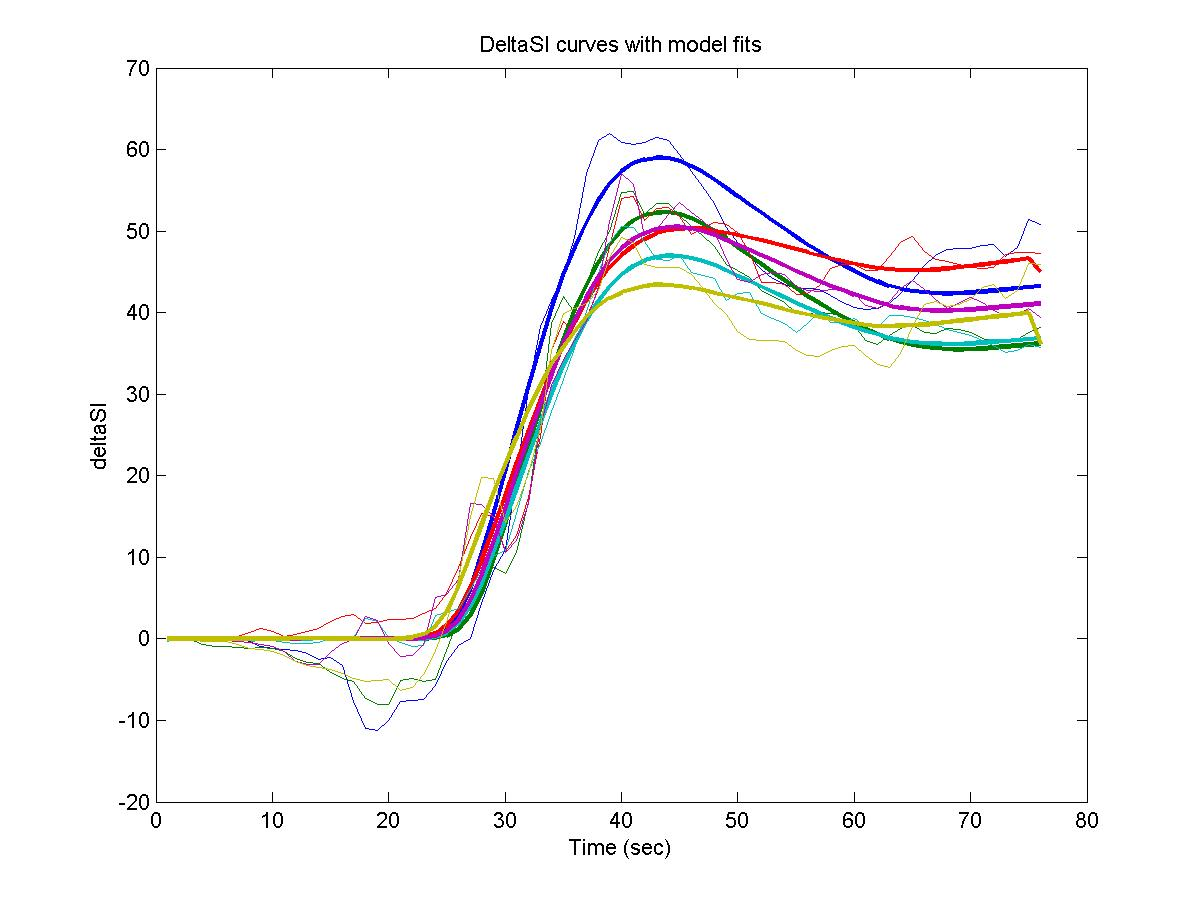
\includegraphics[width=40mm]{Figures/Results_jpg_DZnomask/MoCo_08_DZNoMask_Stress_Fit.jpg} \\
    \rotatebox{90}{\bf \,\,\,\,\,\,\,\,\,\,\,\,\,MoCo\_09} & 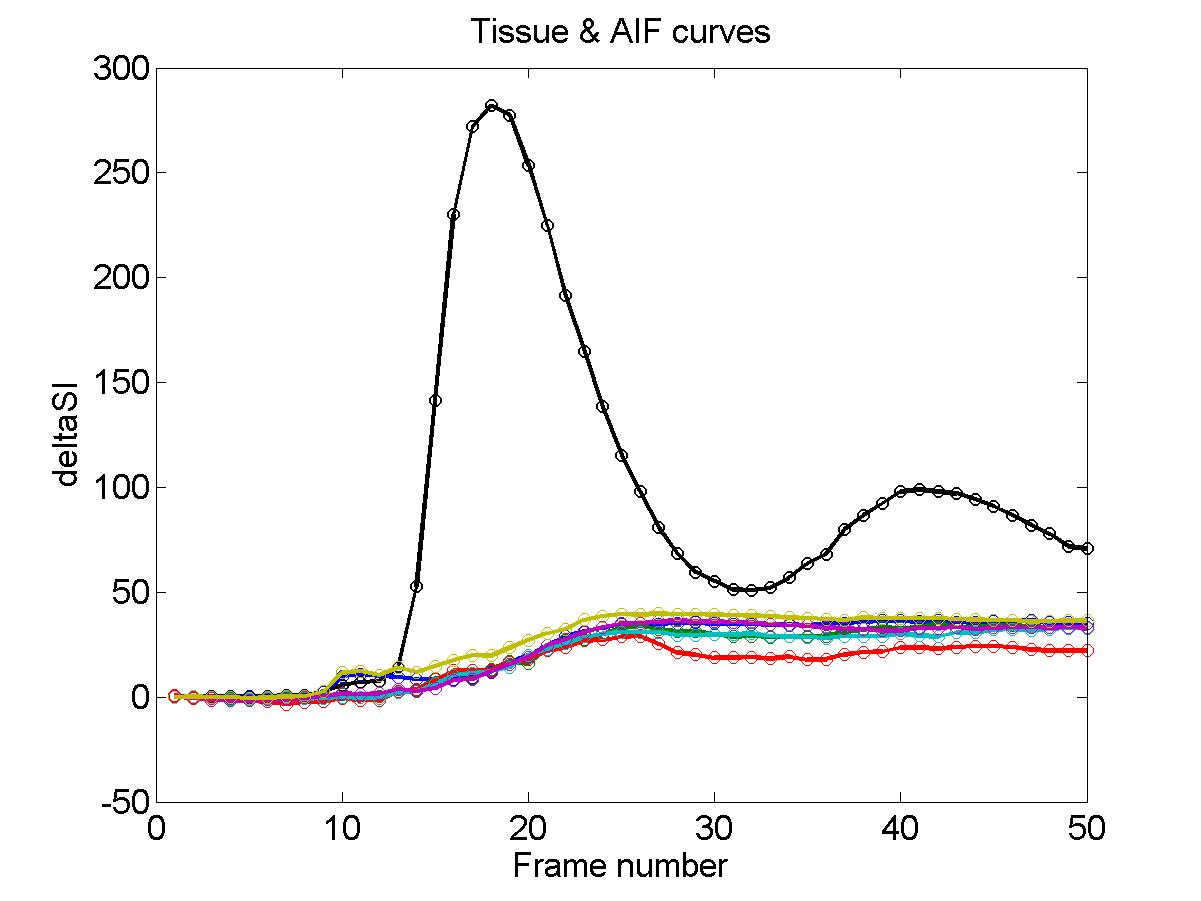
\includegraphics[width=40mm]{Figures/Results_jpg_DZnomask/MoCo_09_DZNoMask_Rest_Curve.jpg} 
    \hspace{-5mm} &
    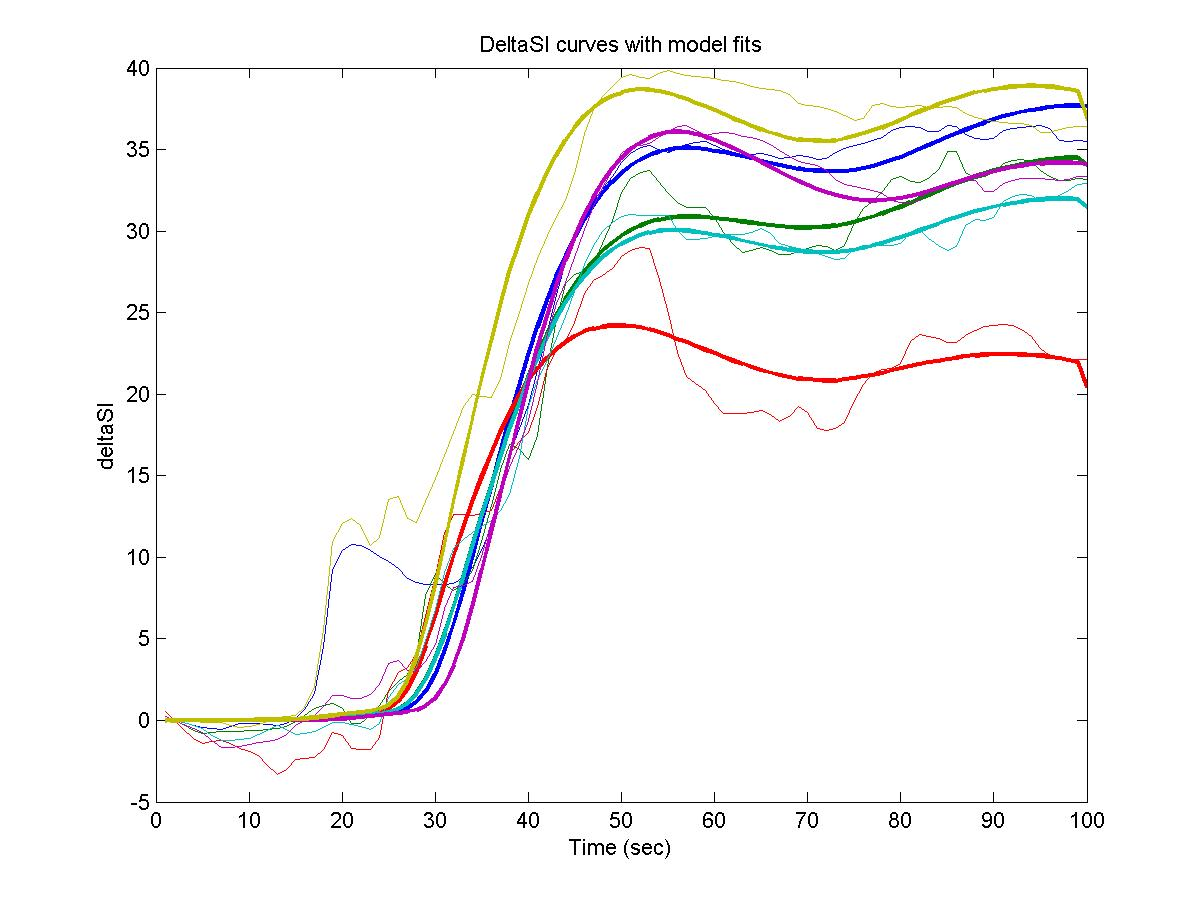
\includegraphics[width=40mm]{Figures/Results_jpg_DZnomask/MoCo_09_DZNoMask_Rest_Fit.jpg} 
    \hspace{-5mm} &
    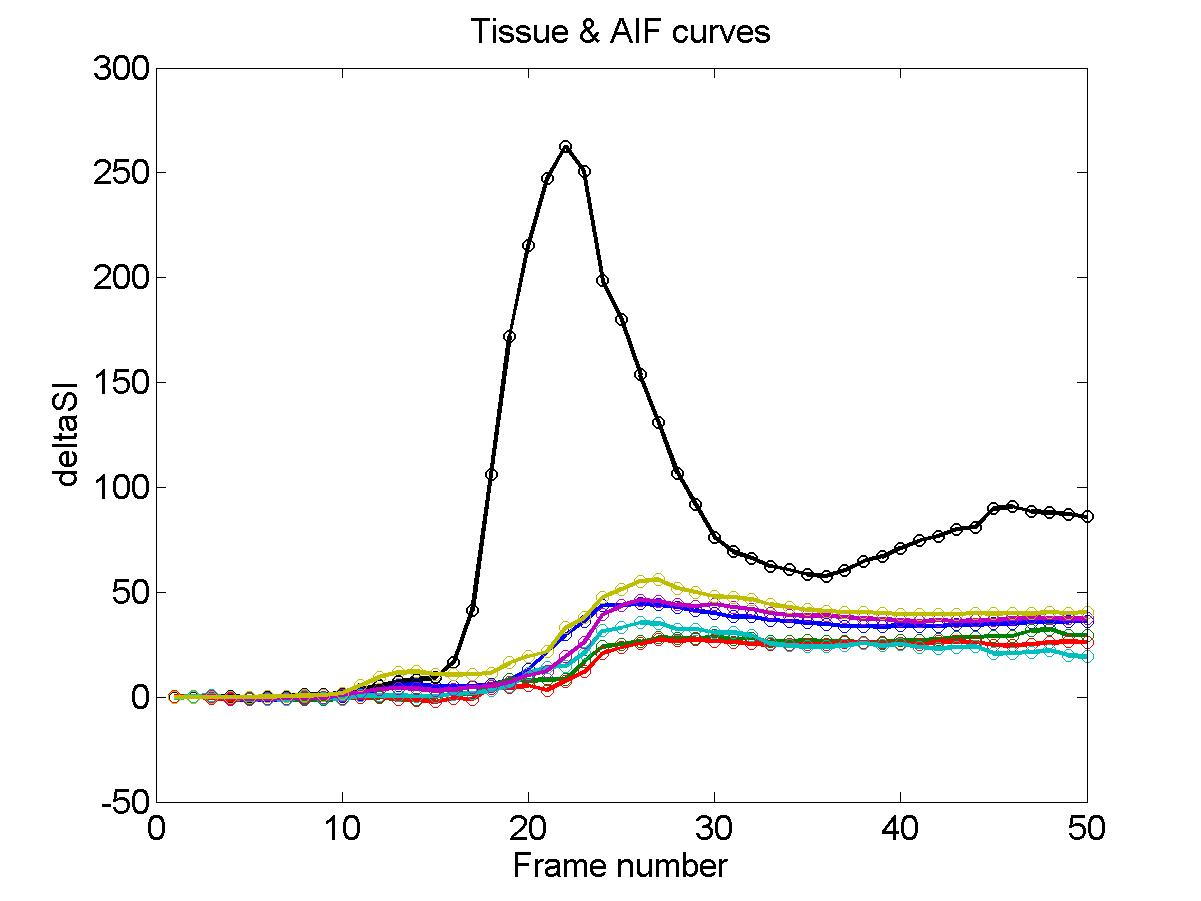
\includegraphics[width=40mm]{Figures/Results_jpg_DZnomask/MoCo_09_DZNoMask_Stress_Curve.jpg} 
    \hspace{-5mm} &
    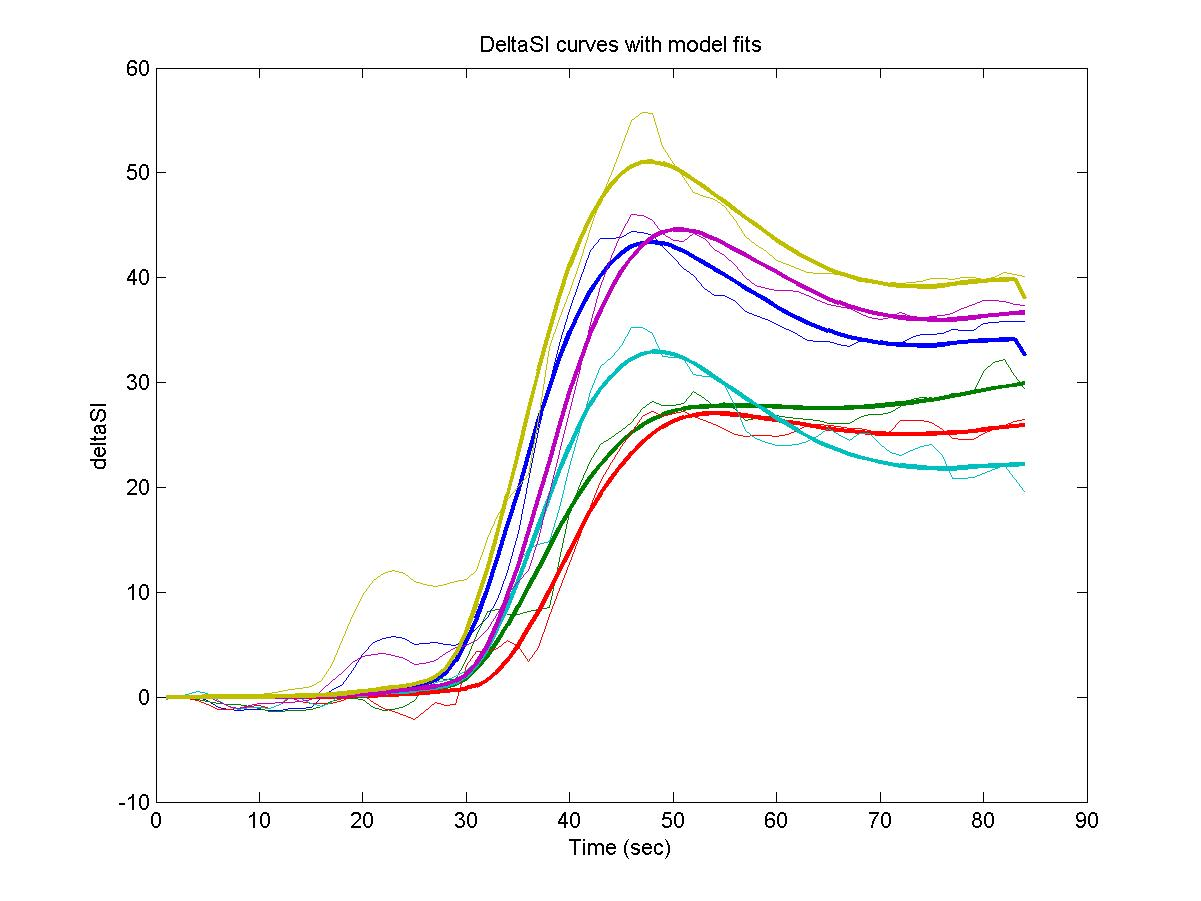
\includegraphics[width=40mm]{Figures/Results_jpg_DZnomask/MoCo_09_DZNoMask_Stress_Fit.jpg} \\
    \rotatebox{90}{\bf \,\,\,\,\,\,\,\,\,\,\,\,\,MoCo\_10} & 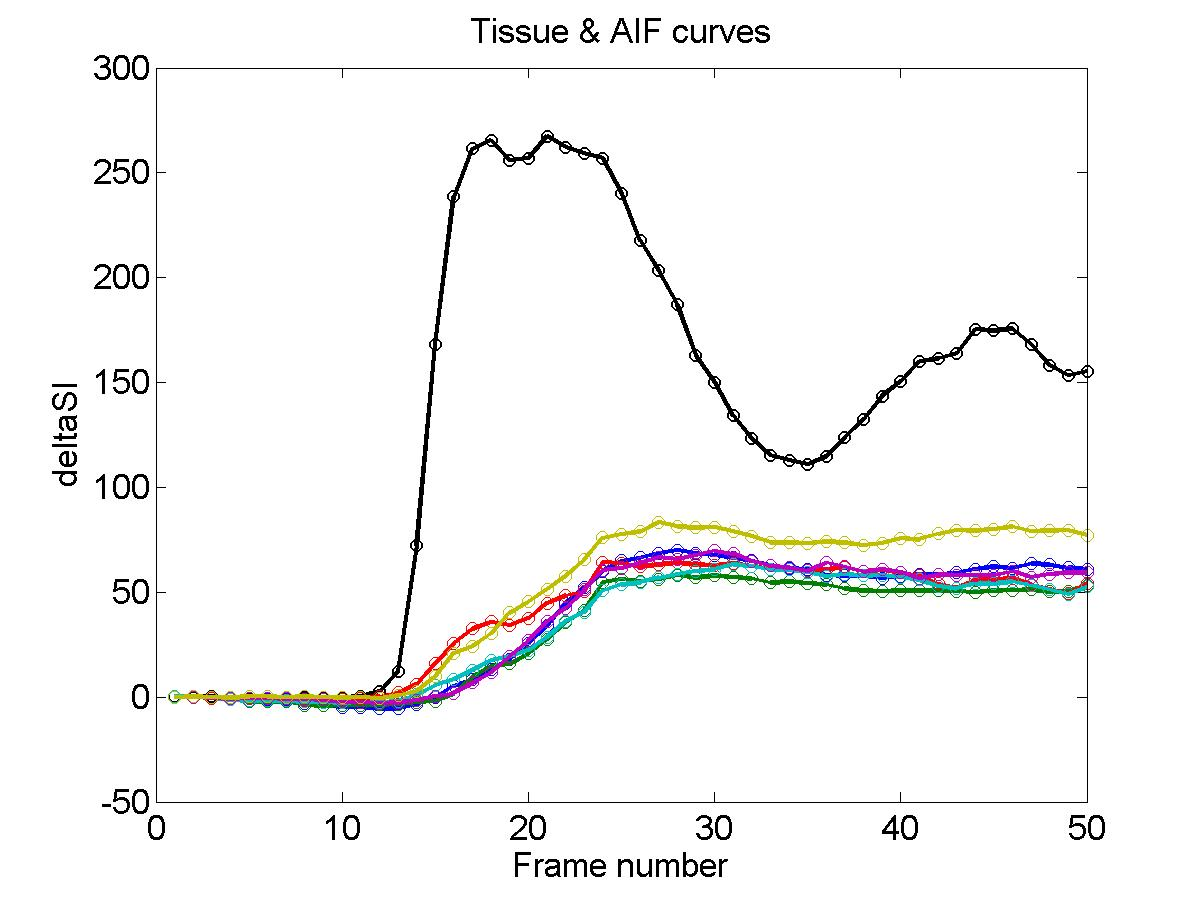
\includegraphics[width=40mm]{Figures/Results_jpg_DZnomask/MoCo_10_DZNoMask_Rest_Curve.jpg} 
    \hspace{-5mm} &
    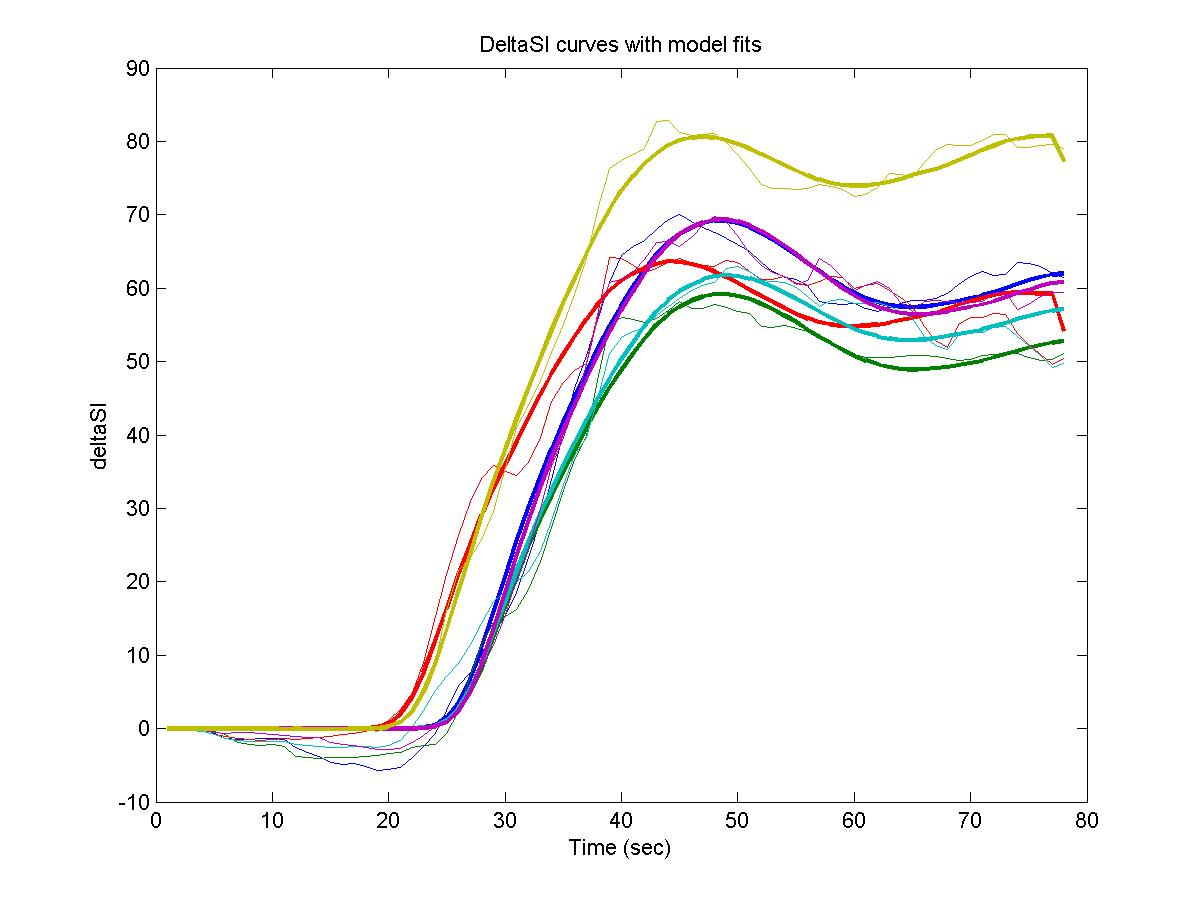
\includegraphics[width=40mm]{Figures/Results_jpg_DZnomask/MoCo_10_DZNoMask_Rest_Fit.jpg} 
    \hspace{-5mm} &
    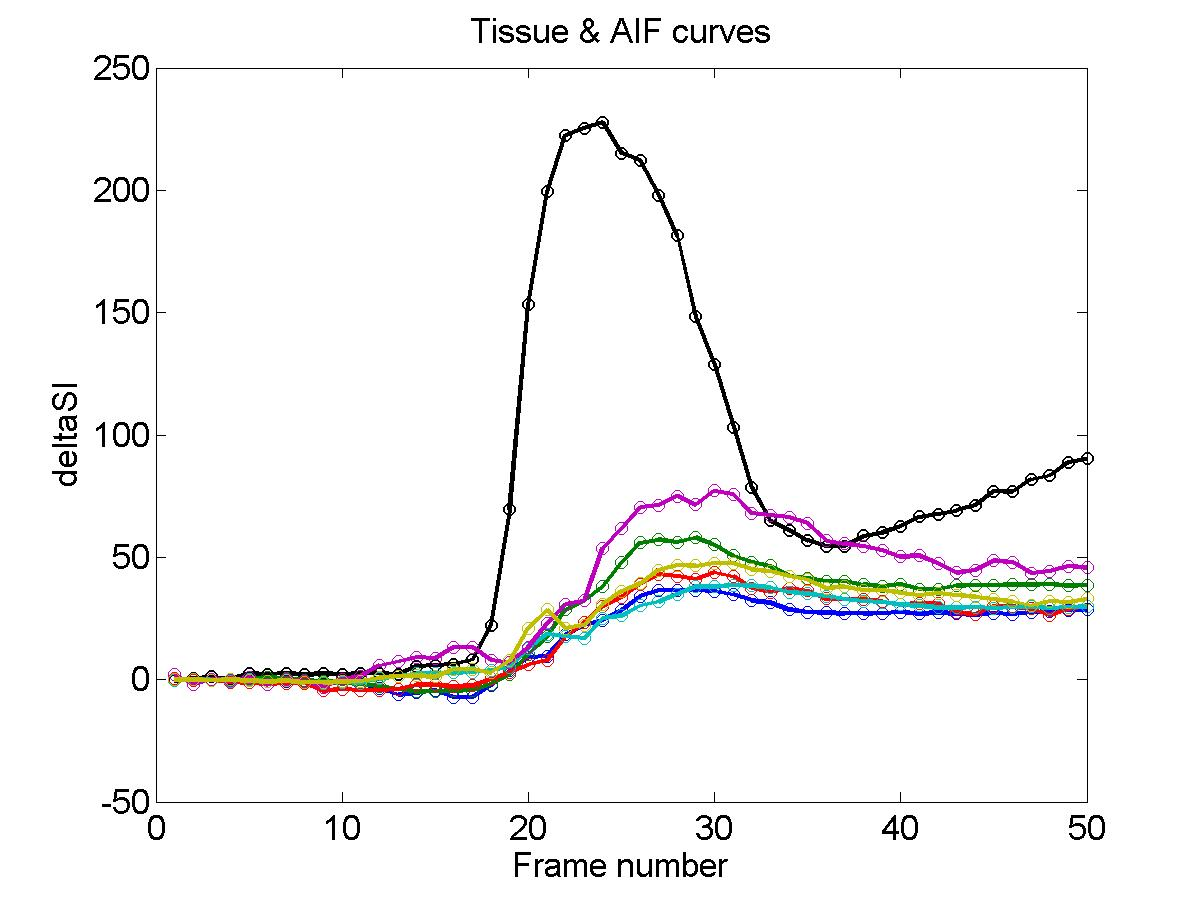
\includegraphics[width=40mm]{Figures/Results_jpg_DZnomask/MoCo_10_DZNoMask_Stress_Curve.jpg} 
    \hspace{-5mm} &
    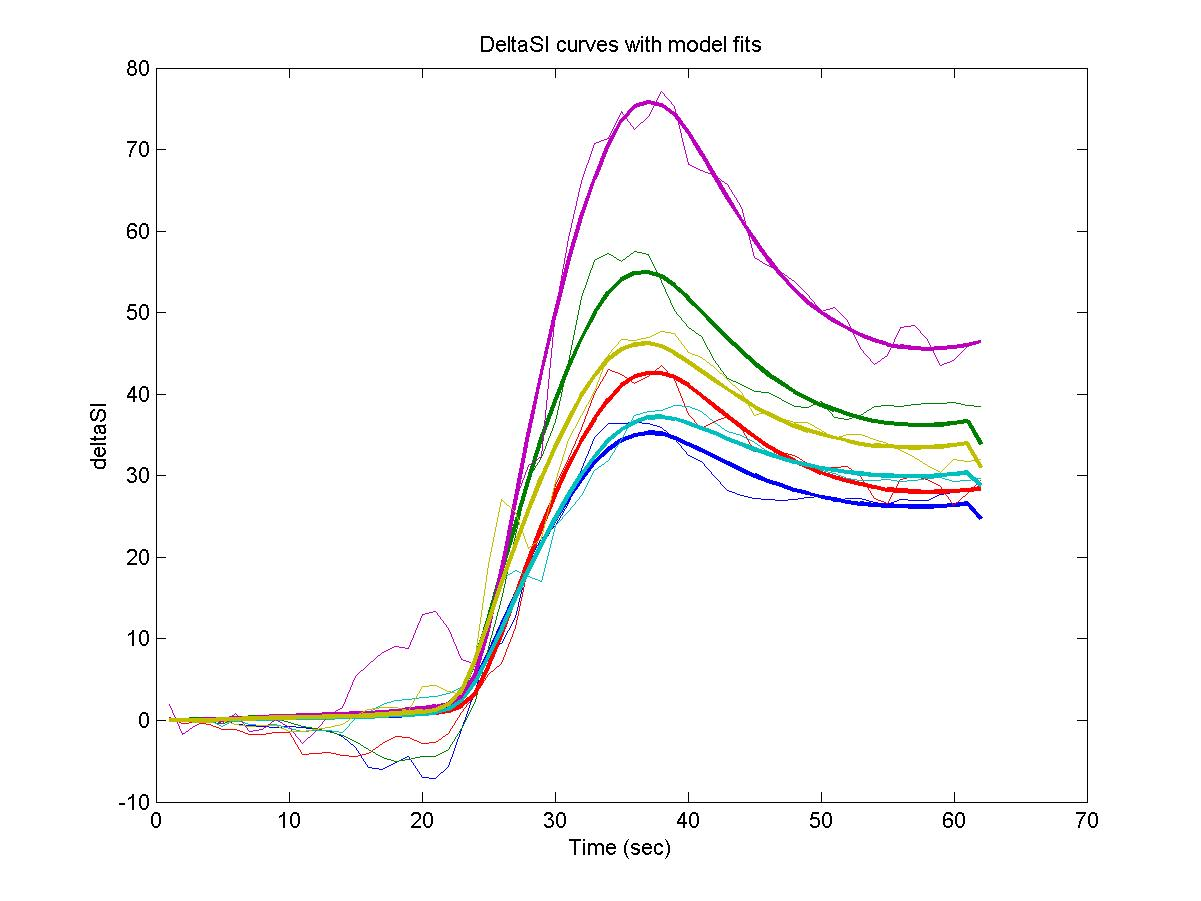
\includegraphics[width=40mm]{Figures/Results_jpg_DZnomask/MoCo_10_DZNoMask_Stress_Fit.jpg} \\
  \end{tabular}
  }
  \caption{Validation time curves consisting of tissue and arterial input function time plots 
  for the gated data sets 6--10.}
  \label{fig:gated2}
\end{figure}
    
    
\begin{figure}
 \makebox[\textwidth][c]{
   \begin{tabular}{rcc}
    \rotatebox{90}{\bf \qquad\qquad Ungated} & 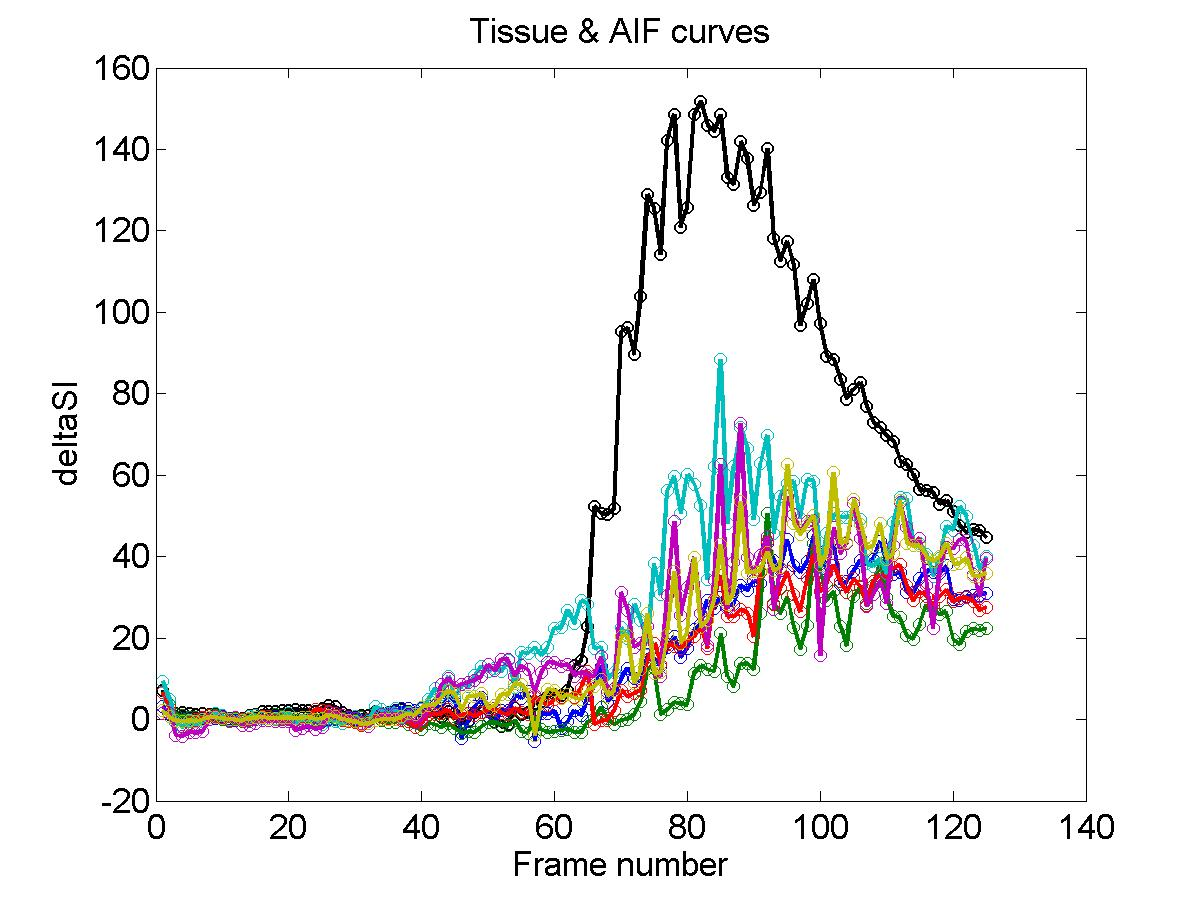
\includegraphics[width=60mm]{Figures/Results_jpg_DZnomask/MoCo_Ungated_DZNoMask_Rest_Curve.jpg} 
    \hspace{-5mm} &
    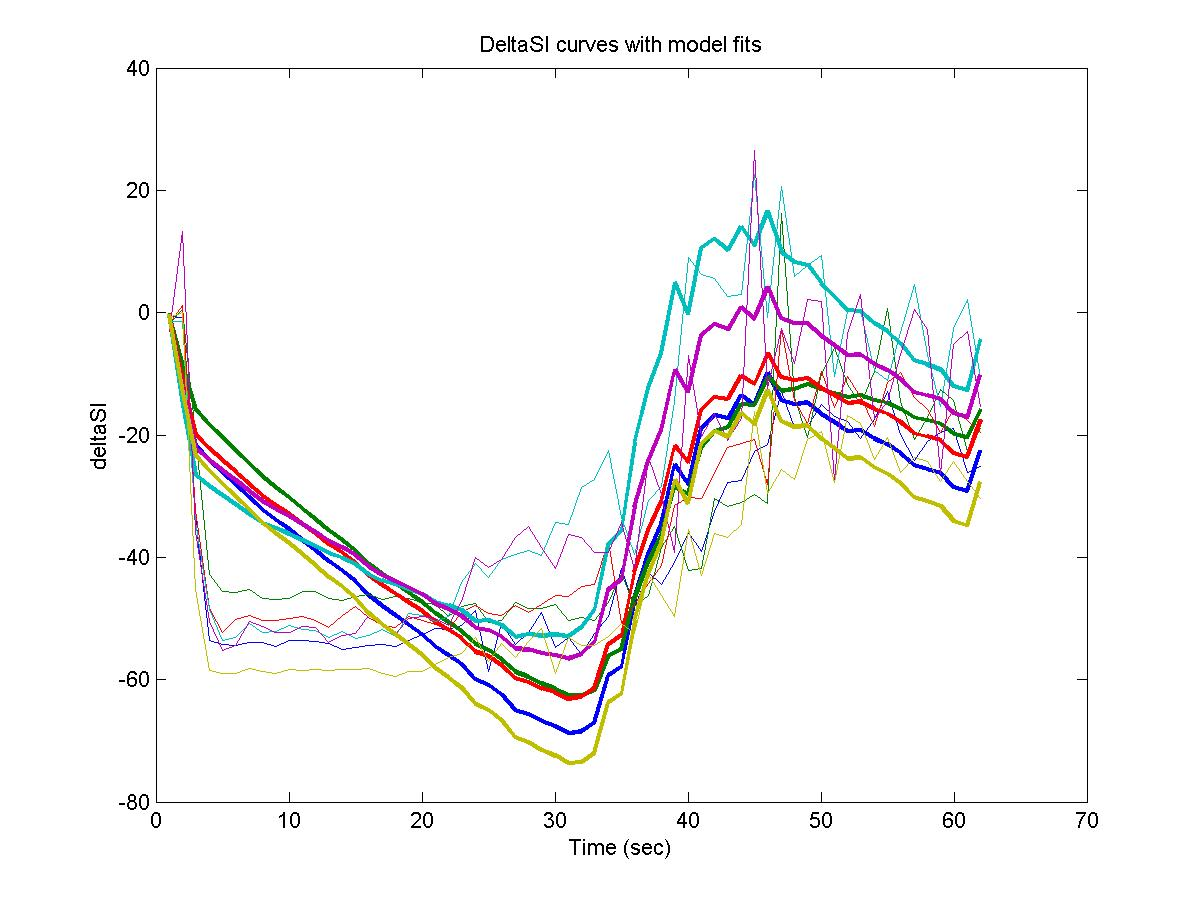
\includegraphics[width=60mm]{Figures/Results_jpg_DZnomask/MoCo_Ungated_DZNoMask_Rest_Fit.jpg} 
  \end{tabular}
  }
  \caption{Validation time curves consisting of tissue and arterial input function time plots 
  for the ungated data set.}
  \label{fig:ungated}
\end{figure}



\section{Discussion and Conclusions}
Although an improvement over the non-corrected image data, our motion
correction technique is far from being a definitive solution. Confounds
such as noise and lack of contrast caused errors during the alignment
optimization over all subjects.  This was particularly the case for 
the ungated data set for which the same parameters were applied as with the 
gated data.  Considering the different motion characteristics between the two
types of data, the heuristically-chosen optimal parameters selected for the
latter might be suboptimal for the former.  Further investigation with 
additional ungated data would be necessary for tuning a different, targeted set
of parameters.

The general principle of incorporating prior knowledge 
to improve solution strategies is definitely an avenue we are pursuing
for future work.  One extension we are currently investigating is the 
use of optimal shape and intensity templates derived from the subject
image data.  By coalescing similar images into subgroups of optimal templates and calculating
the transforms between them, optimal transformation paths between images can be found
using graph-theoretic methods.

\bibliographystyle{splncs03}
\bibliography{references}

\end{document}
